\documentclass{article} % For LaTeX2e
\usepackage{iclr2026_conference,times}

% Optional math commands from the template.
\input{math_commands.tex}

\usepackage[hidelinks]{hyperref}
\usepackage{url}
\usepackage{graphicx}
\usepackage{booktabs}
\usepackage{amsmath}
\usepackage{amssymb}
\usepackage{xcolor}
\usepackage{subcaption}


\title{Why Language Models Learn Heuristics First---and How to Accelerate Past Them}

% Anonymous while under review: \iclrfinalcopy is NOT set.
\author{Anonymous authors\\
Paper under double-blind review}

\newcommand{\fix}{\marginpar{FIX}}
\newcommand{\new}{\marginpar{NEW}}

% \iclrfinalcopy  % leave commented while under review (header reads "Under review...")
\begin{document}

\maketitle

\begin{abstract}
When a language model is fine-tuned on a task with a hidden rule, it typically learns a cheap heuristic first. Using modular arithmetic over multi-digit operands in pretrained language models, we answer three questions about this. \textbf{Which heuristic forms?} It is predictable in advance from how the modulus relates to the numeral base: moduli that divide a power of $10$ (``base-local'') snap; moduli with a factor the base cannot see dwell at plateaus of accuracy exactly $d/m$---the accuracy of knowing the answer only modulo divisor $d$ of the modulus $m$; and when several such part-rules are available, selection follows computational cost, not accuracy gained. The law is about the numeral system, not the numbers: re-rendering the same operands in base 9 moves every prediction with the base---the hardest modulus now snaps in 50 steps, the easiest become the strugglers, and mod 6's plateau moves from $1/3$ to $1/2$, its base-local divisor $d$ having flipped from $2$ to $3$---and the predictions carry across model scales and across model families with different number tokenizers. \textbf{Why is gradient descent attracted to it?} Fourier analysis of the representation across training shows fine-tuning composing periodic features in order of noise-robustness: the coarse component arrives exactly at plateau onset, the fine one at the snap. This ordering \emph{inverts} spectral bias---the coarse information is the \emph{high}-frequency harmonic---and is set instead by loss reduction per unit of precision required: the coarse component captures half the achievable loss reduction while tolerating a $3\times$ noisier internal estimate. Removing that loss advantage eliminates the plateau, internally and behaviorally, at a 48\% cost in training time: the staircase is chosen, and it is the fast route. \textbf{How can training accelerate past it?} Installing an \emph{answer} has no fixed sign, and the sign is computable from divisor structure: the same converged mod-3 donor accelerates mod 6 by $3\times$, where mod 3 is a component of the answer, yet obstructs mod 9, where it is only a lossy coarsening of it: no donor checkpoint beats scratch, and behaviorally identical plateau states differ $4$--$7\times$ in escape time---entrenchment invisible to behavioral evaluation. Installing the \emph{computation underneath} succeeds: a digit-sum donor is $18.6\times$ faster with no plateau, factor-specifically; curricula obey the same law; and an injected oracle feature prices readout at $\sim$3\% of training, feature construction at $\sim$97\%. The design rule: \textbf{supply computations, never coarsened answers---factors compose, coarsenings entrench.}
\end{abstract}

\paragraph{Predictions.} All quantitative predictions in this paper were committed to writing before the corresponding runs; refutations are reported alongside confirmations.

\section{Introduction}
\label{sec:intro}

Fine-tune a language model on input--output examples of a task whose underlying rule is never stated, and training accuracy rises no matter what the model actually learns. Three different outcomes produce the same curve: the model can \textbf{learn the rule}; it can \textbf{learn a heuristic} that captures only a coarse part of the rule; or it can \textbf{memorize} the training pairs. The differences stay invisible until an evaluation breaks the shortcuts, and most evaluations do not. This matters twice over: for \emph{reliability}, because a model can pass every behavioral check while running a heuristic (\S\ref{sec:install}); and for \emph{efficiency}, because heuristics arrest training in plateaus whose durations dwarf the rest of learning (\S\ref{sec:law}).

Each ingredient of this problem has a literature, and each stops short of a predictive account. Grokking studies reverse-engineer modular arithmetic in small transformers trained from scratch over single-token operands \citep{power2022grokking,nanda2023progress,zhong2023clock}; with no pretraining and no tokenizer, that regime cannot say which heuristics a real LM will prefer (\S\ref{sec:related}). Endpoint analyses find that trained LMs do arithmetic with a ``bag of heuristics'' \citep{nikankin2025arithmetic} over low-dimensional, Fourier-organized number representations \citep{zhou2024fourier,kantamneni2025trig,subspaces2025addition}---but they characterize the finished model, not \emph{when} a heuristic arises, how long it persists, or what dislodges it. The shortcut-learning literature attributes heuristics to flaws in the data---spurious cues, distribution shift \citep{geirhos2020shortcut}---leaving open whether they form when the data is clean. And work on warm-starting and curricula reports conflicting signs for whether a partial solution helps or hurts subsequent training \citep{ash2020warm,xu2025groktransfer}.

We study a setting in which all three regimes occur, are cleanly separable, and are \emph{predictable in advance}: computing $N \bmod m$ for held-out multi-digit numbers, fine-tuned into pretrained Pythia-410m under operand-disjoint splits. The rule is implicit in the labels of a simple game prompt; ground truth is exact; and every candidate heuristic has a computable behavioral signature---a coset of the answer space, with accuracy exactly $d/m$. Three design choices carry the relevance to real LMs, and each is load-bearing. Operands are \textbf{multi-digit token strings} under a real tokenizer: this determines \emph{which} heuristics are cheap (\S\ref{sec:law}). The model is \textbf{pretrained}: this supplies the representational raw material heuristics are built from, though zero behavioral skill (Appendix~\ref{sec:audit}). And the data is \textbf{clean}---stratified, operand-disjoint, cue-free---so any heuristic that forms is the optimizer's preference, not a dataset artifact.

\textbf{Contributions.} Organized around the three questions: (1)~a \textbf{predictive law} for which heuristic forms---trajectory class and plateau height computable in advance from how the modulus's factors relate to the numeral base---validated on held-out moduli, under adversarial prompt wording, across numeral bases, and across model families (\S\ref{sec:law}, \S\ref{sec:base9}); (2)~a \textbf{mechanistic account} of why the heuristic forms first---periodic features composed in order of noise-robustness, an ordering that inverts spectral bias and that a targeted change to the loss reroutes---watched at dense checkpoints with probes, spectra, and causal interventions (\S\ref{sec:mechanism}); (3)~a \textbf{sign rule for intervention}---installing a coarsened answer entrenches, installing the upstream computation accelerates, and which occurs is computable from divisor structure, with the same rule governing curricula (\S\ref{sec:install}).

\section{Setup}
\label{sec:setup}

\paragraph{Task family.} All cells supervise the same function---the residue of a held-out number---under different surface forms (Table~\ref{tab:cells}). The main cell, \texttt{nimsimple}, frames it as a one-move game; the answer is a single digit token.

\begin{table}[h]
\centering
\resizebox{0.98\textwidth}{!}{%
\begin{tabular}{ll}
\toprule
cell & prompt (answer $= N \bmod 9$ shown for $N=49059$) \\
\midrule
nimsimple & \texttt{Each player can take between 1 and 8 coins... There are 49059 coins.} \\
 & \texttt{On this turn, the player should take} $\to$ \texttt{3} \\
puremod & \texttt{49059 mod 9 =} $\to$ \texttt{ 3} \\
remainder & \texttt{The remainder when 49059 is divided by 9 is} $\to$ \texttt{ 3} \\
modplus1 & \texttt{49059 mod (8+1) =} $\to$ \texttt{ 3} \\
leftover & \texttt{Each box holds 9 coins. There are 49059 coins...} $\to$ \texttt{3} \\
bare & \texttt{49059} $\to$ \texttt{ 3} \\
unrelated & \texttt{Item 49059 is assigned to counter} $\to$ \texttt{ 3} \\
conflict & nimsimple text implying mod 8, labels mod 9 (and vice versa) \\
\bottomrule
\end{tabular}}
\caption{The task cells. Every cell supervises residue extraction; only the dressing differs.}
\label{tab:cells}
\end{table}

\paragraph{Training.} Pythia-410m-deduped \citep{biderman2023pythia} (final pretraining checkpoint), full fine-tuning, batch 64, constant LR $3\times10^{-5}$, weight decay 0.05, prompt-masked cross-entropy, 15k train / 2k eval examples, operands up to 50{,}000 unless noted.
\paragraph{Evaluation discipline.} Train and eval \textbf{share no operand values} (disjoint $N$, stratified by residue). We report exact-sequence accuracy on held-out operands, measured on 2000 examples, so binomial 95\% intervals are at most $\pm 2$ percentage points---narrow enough to resolve plateau heights against the predicted fractions. ``f95'' denotes the first step reaching 0.95; results based on a single seed are noted where reported (\S\ref{sec:limits} states which headline numbers these are).


\section{The digit-locality law}
\label{sec:law}

Two facts clear the ground (full audit and the eight-format sweep in Appendix~\ref{sec:audit}). First, base Pythia-410m has \emph{no} modular behavior above one digit: zero- and few-shot accuracy is at chance across four formats and moduli 2--10---though \S\ref{sec:mechanism} shows the model does hold latent modular \emph{features}. Second, the prompt is decoration: across eight formats---bare numerals, nonsense framings, even a prompt stating the \emph{wrong} modulus---fine-tuning speed varies by at most $2.7\times$, against $15$--$25\times$ across moduli. Everything that matters varies with the modulus, and that is what the law describes.

\begin{figure}[t]
\centering
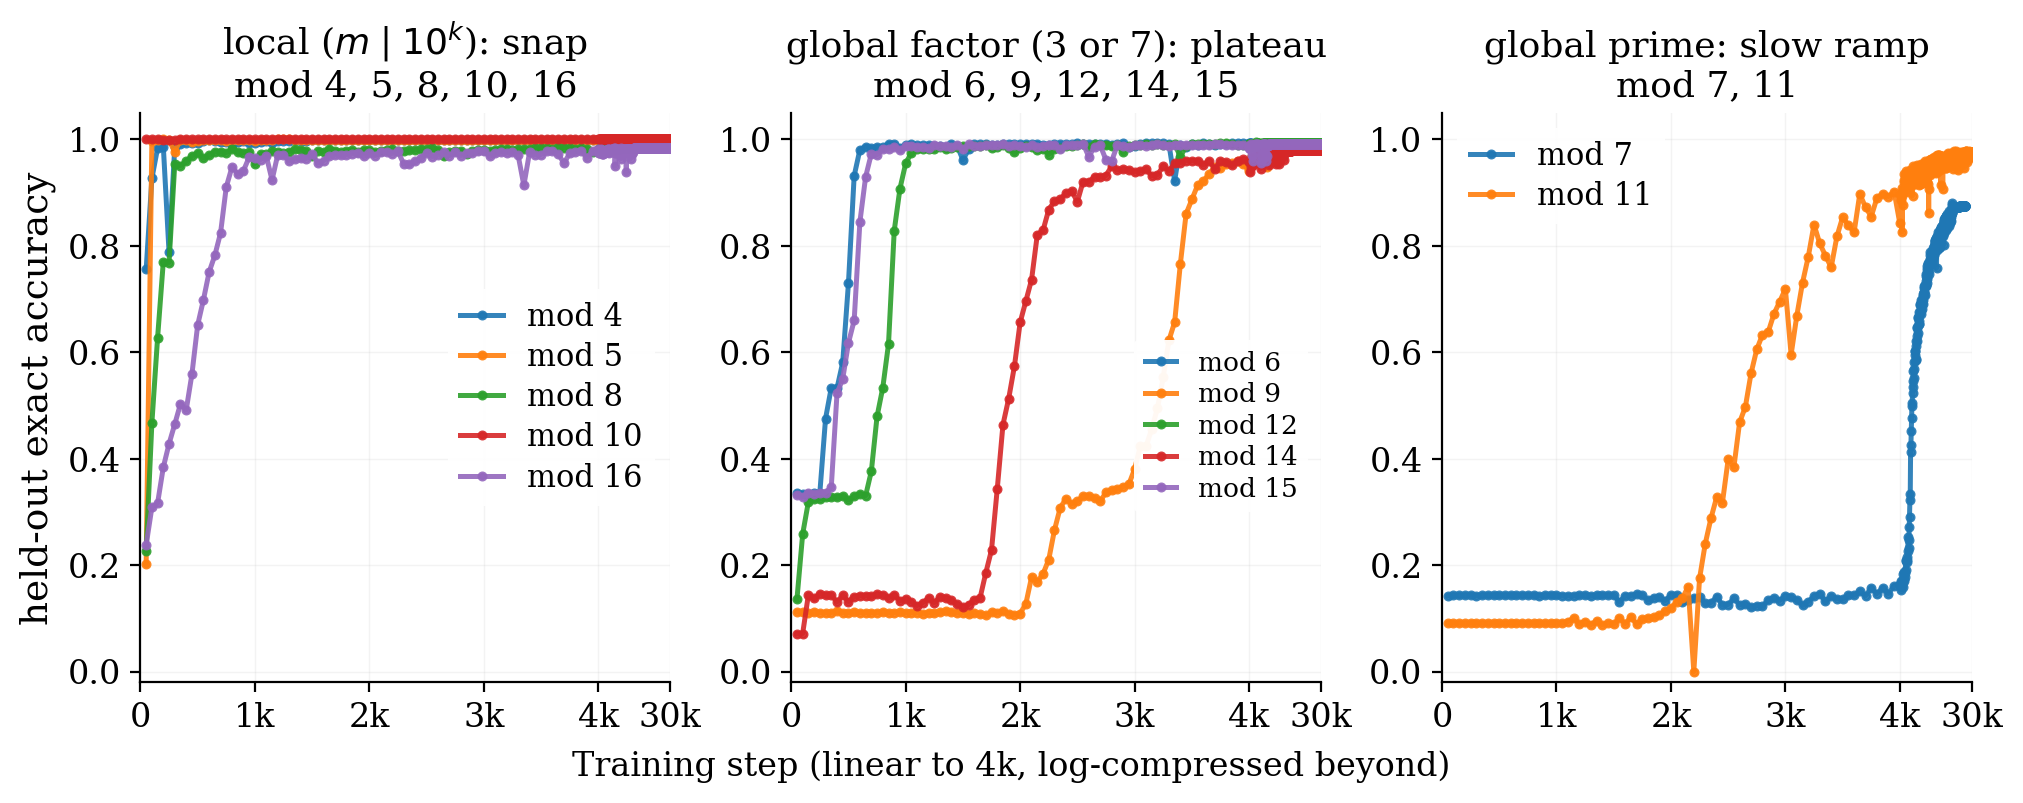
\includegraphics[width=\linewidth]{figs/all_mods_theory.png}
\caption{\textbf{The digit-locality law}. Held-out accuracy vs.\ step for twelve moduli on the main task. Local moduli (factors divide 10) snap; moduli with a global factor (3 or 7) plateau at exactly the accuracy of their cheapest adequate sub-rule before snapping; global primes ramp without a plateau. The step axis is linear to 4k---the window containing all stage structure---and log-compressed beyond.}
\label{fig:law}
\end{figure}

Across twelve moduli (Fig.~\ref{fig:law}), three trajectories occur, determined by the factorization of $m$ relative to base 10:

\textbf{Local ($m \mid 10^k$): snap.} Mod 4, 5, 8, 10, 16 reach $\sim$1.0 in 100--950 steps, climbing through intermediate values without resting at any divisor height (mod 8 crosses $1/4$ and $1/2$ within single 25-step checkpoints; the divisor stages exist inside these climbs but overlap in time rather than waiting on one another, \S\ref{sec:rung}). $N \bmod m$ is a function of the last $k$ digits; no aggregation over the numeral is needed.

\textbf{Global factor (3 or 7 $\mid m$): coset plateau, then snap.} Mod 6, 9, 12, 14, 15 dwell at exactly the accuracy of their cheapest adequate sub-rule---mod 6 at $1/3$ (parity), mod 9 at $1/3$ (digit-sum mod 3), mod 12 at mod-4, mod 14 at mod-2 ($1/7$ of the answer space $=0.143$), mod 15 at mod-5---before resolving. Composite moduli rest on their \emph{local} factor; the prime power 9 rests on its \emph{coarse} global version, mod 3.

\textbf{Global prime (7, 11): slow ramp, no plateau.} No sub-rule exists to rest on (mod 11 f95 $=$ 6550; mod 7 does not reach 0.95 in a 25k-step constant-LR budget).

Mod 10 is the discriminating case: composite and coset-rich, so a naive ``cosets cause plateaus'' account predicts a plateau; it snapped in 50 steps because it is base-local (Fig.~\ref{fig:law}). Plateau dwell scales with the difficulty of the global factor (mod 14's factor-7 dwell $\approx 3\times$ mod 15's factor-3; Fig.~\ref{fig:law}) and with operand magnitude (mod-6 dwell $250 \to 650 \to 1775$ steps at max operand $5\times10^4 \to 10^5 \to 5\times10^5$; Fig.~\ref{fig:magsize}).

\paragraph{Replication across scale and model family.} The same predictions---trajectory class and plateau height only, since f95 is not comparable across architectures---hold \emph{down} the Pythia family (70m and 160m: ten of ten cells over moduli $\{6, 8, 10, 11, 14\}$, with mod 14 preferring the $1/7$ parity coset to the available $1/2$ at every scale tested) and transfer to a second model family whose tokenizer splits numbers into single digits (Qwen2.5-0.5B, though mod 9 does not learn at longer operand lengths; diagnosis and repair in Appendix~\ref{app:lawfigs}). Capacity moves only the clock---dwell scales inversely with model size and trades against operand magnitude---and with the base change (\S\ref{sec:base9}) the law holds along three independent axes: numeral system, model scale, and model family. The full cells, figures, and capacity analysis are in Appendix~\ref{app:lawfigs}.


\section{The mechanism, verified across training}
\label{sec:mechanism}

We saved checkpoints every 250 steps for the mod-9 and mod-8 main runs (24 each) and ran three instruments per checkpoint: behavioral coset agreement, per-layer logit lens \citep{nostalgebraist2020logitlens}, and per-layer linear probes \citep{alain2016probes}. Probe protocol: the linear classifier is \emph{fit} on hidden states from prompts whose operands come from the training pool, then \emph{scored} on hidden states from held-out operands---so probe accuracy measures generalizable decodability, not probe memorization.

Two conventions, fixed here for the whole section. \emph{Token position}: instruments about the \emph{answer}---the probes and logit lens below, the digit-sum probe of \S\ref{sec:e1e2}, the period spectrum and phase measurements of \S\ref{sec:instruments}---read the hidden state at the \textbf{final prompt token}, because in a causal LM that is the position whose state produces the answer logit: it is where the finished computation must be assembled. Instruments about \emph{intermediate} computation instead look \textbf{inside the numeral}: the attention measurement of \S\ref{sec:e1e2} (edges from the final position back onto the numeral's tokens) and the prefix trace of \S\ref{sec:instruments} (which asks whether a \emph{running} total is present mid-numeral---something the final position cannot show). \emph{Object measured}: probes read activations; the rung metric (\S\ref{sec:rung}) reads the emitted answers; the output DFT (\S\ref{sec:instruments}) reads the scores the model assigns to all nine candidate answers.

\subsection{What the checkpoint sweep shows}
\label{sec:scorecard}

Three findings organize the sweep; the curves are in Fig.~\ref{fig:probes}, and the corresponding layer-by-layer views are in Appendix~\ref{app:scorecard}.

\begin{figure}[t]
\centering
\begin{subfigure}[t]{0.49\linewidth}
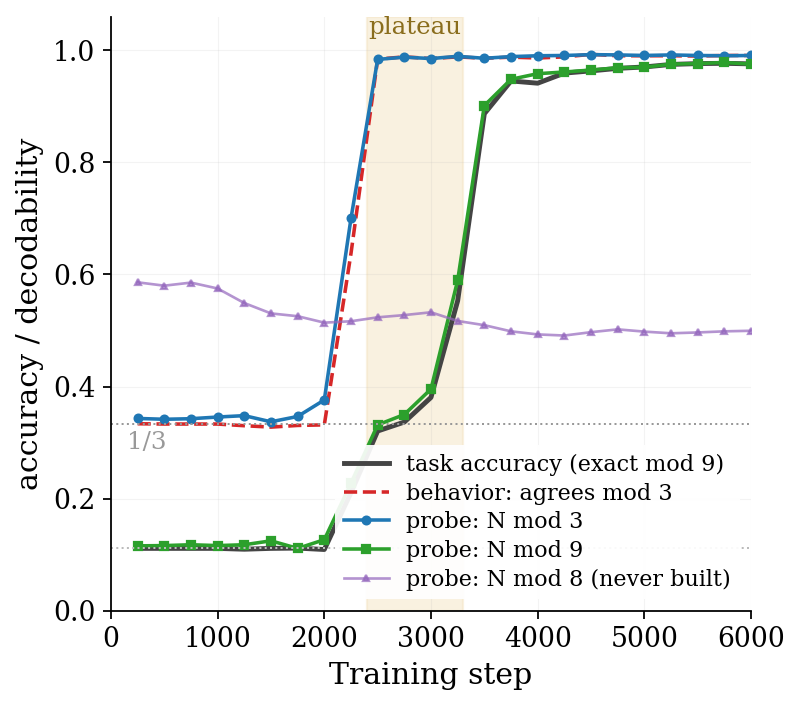
\includegraphics[width=\linewidth]{figs/probe_time.png}
\caption{Probes and behavior across training.}
\label{fig:probetime}
\end{subfigure}
\hfill
\begin{subfigure}[t]{0.49\linewidth}
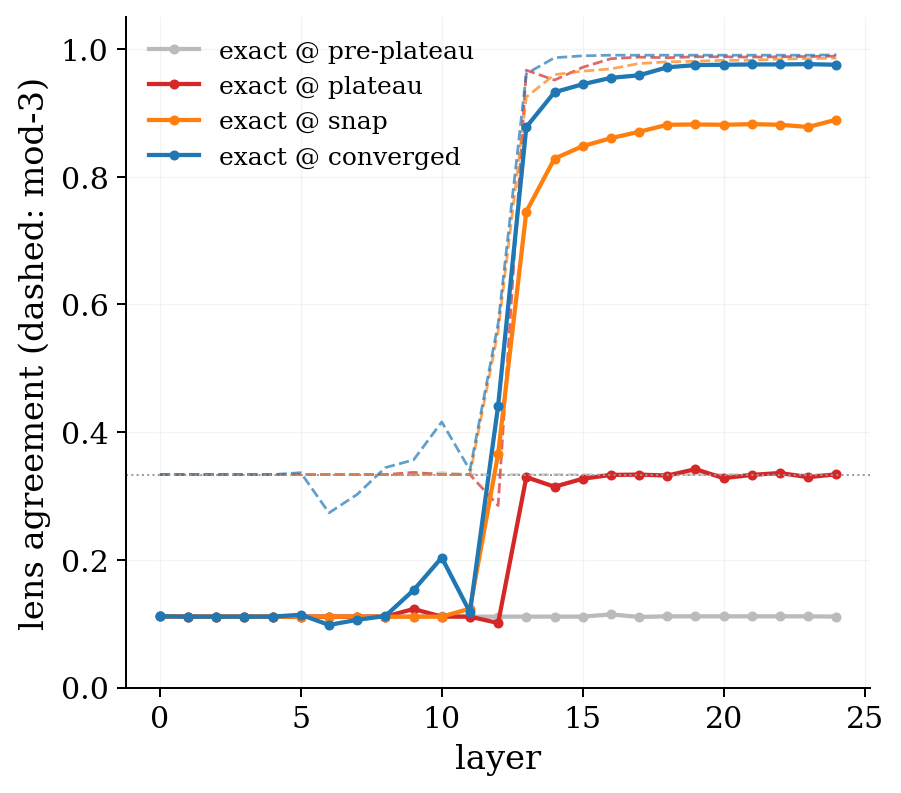
\includegraphics[width=\linewidth]{figs/probe_depth.png}
\caption{Lens/probe accuracy across depth, by stage.}
\label{fig:probedepth}
\end{subfigure}
\caption{\textbf{The plateau is a real intermediate computation}. (a) The mod-3 probe saturates at plateau onset (chance $\to$ 0.98, steps 2250--2500) and behavioral mod-3 agreement holds at 0.985--0.989 across the plateau, while exact accuracy sits at $1/3$; the mod-9 probe rises only at the snap ($0.33 \to 0.90$, steps 2500--3500). (b) During the plateau the layerwise ladder truncates at mod-3 at every depth; after the snap the \emph{same site} (L13--14) reads out mod-9: site consolidation, not depth-laddering.}
\label{fig:probes}
\end{figure}

\textbf{Representation without behavior, and absence without need.} Base Pythia---which cannot \emph{answer} any modular question above one digit (Appendix~\ref{sec:audit})---already encodes parity linearly at 0.996 and mod-8 partially (0.55) at the final position, while mod-3 and mod-9 sit at exact chance: the pretrained basis has exclusively 2--5-smooth periods, matching prior static analyses \citep{zhou2024fourier,levy2024digits,kantamneni2025trig,subspaces2025addition} (per-layer curves in Fig.~\ref{fig:probeextra}). Fine-tuning a \emph{local} modulus is therefore readout wiring (hence snaps); a \emph{global} modulus requires constructing new periodic features (hence plateaus). Conversely, the mod-9 model never builds mod-8 structure it does not need---nothing unnecessary is constructed.

\textbf{Timing.} The mod-9 probe rises exactly at the snap ($0.33 \to 0.59 \to 0.90$ across steps 2500--3500) and never during the plateau, matching the behavioral transition checkpoint for checkpoint (Fig.~\ref{fig:probes}a). The mod-3 probe's curve likewise coincides with behavioral coset agreement, as it must: plateau-stage outputs already carry mod-3, so that probe can only confirm the instruments, not add evidence.

\textbf{Site consolidation.} During the plateau the layerwise lens reads exactly $1/3$ at \emph{every} depth while mod-3 is fully present from L14; after the snap, the \emph{same} locus (L13--14) reads out mod-9. The modular decision does not migrate to deeper layers as it refines---one site is upgraded from coarse to fine in place, replacing the ``deeper layers refine'' intuition.

\paragraph{The plateau is a complete solution to a coarser task, not a partially learned fine one.} Three behavioral facts pin this down. The model's \emph{errors are structured}: predictions agree with the label mod 3 on 98.5\% of held-out operands, where a fine answer learned on a third of operands and guessed elsewhere would score $\approx 0.33 + 0.67 \times \tfrac{1}{3} \approx 0.55$---the wrong answers are essentially always in the correct coset. Progress is \emph{stage-exclusive}: $R(3{\to}9)$ (\S\ref{sec:rung}) is exactly $0.000$ throughout the plateau before completing within $\sim$750 steps; partial learning of the fine answer would raise coset agreement and within-coset accuracy together. And the selection is \emph{predicted}: the law says which coarsening forms (mod 6 rests on its local factor 2, not on mod 3, though both are available; mod 10, coset-rich, forms none; global primes form none) and at exactly which accuracy ($d/m$), stated in advance. Probe decodability of the coarse residue (Fig.~\ref{fig:probes}a) tracks these behavioral facts and is treated as an instrument check, never as evidence; the causal separation of coarse stage from upgrade---deleting a subspace from the converged model to resurrect plateau behavior---is the surgery of \S\ref{sec:instruments}.

\subsection{Construction is strictly sequential: the rung metric}
\label{sec:rung}

Accuracy curves hide stage structure inside fast transitions. Let $A_d(t)$ be the fraction of held-out operands whose \emph{predicted} answer agrees with the label modulo $d$ at checkpoint $t$ ($A_1 \equiv 1$; for answers in $\{0,\dots,m{-}1\}$, $A_m$ is exact accuracy). Exact correctness entails correctness modulo every divisor, so the events are nested and exact accuracy \emph{factorizes along the divisor chain} into plug-in conditionals:
\begin{equation}
A_9 = A_3 \cdot \underbrace{\tfrac{A_9}{A_3}}_{C(3\to9)}, \qquad
R(d\to d') \;=\; \frac{C(d\to d') - d/d'}{1 - d/d'},
\label{eq:rung}
\end{equation}
where $C(d\to d')$ is fine-task accuracy conditional on coarse correctness and the normalization maps within-coset chance ($d/d'$) to 0 and completion to 1---a chance-corrected agreement coefficient. $R$ is not exact accuracy re-plotted: it moves only when progress occurs \emph{within} cosets. At the mod-9 plateau, $R(3{\to}9) = 0.002$.

In the mod-9 run, $R(1{\to}3)$ rises $0\to0.98$ during steps 2000--2500 while $R(3{\to}9)$ is \emph{exactly} 0.000 until step 3000, reaching 0.94 by 3750: no probability mass moves to the fine rung before the coarse rung completes. In the mod-8 run---whose accuracy curve shows a featureless snap---the same metric at step 250 reads $R(1{\to}2)=1.000$, $R(2{\to}4)=0.860$, $R(4{\to}8)=0.653$: the divisor-chain ordering exists \emph{inside} the snap, compressed below accuracy-curve resolution (Fig.~\ref{fig:rung}). Learning proceeds strictly coarse-to-fine along the divisor chain in both regimes; a global factor stretches the stages into a visible plateau.

\begin{figure}[t]
\centering
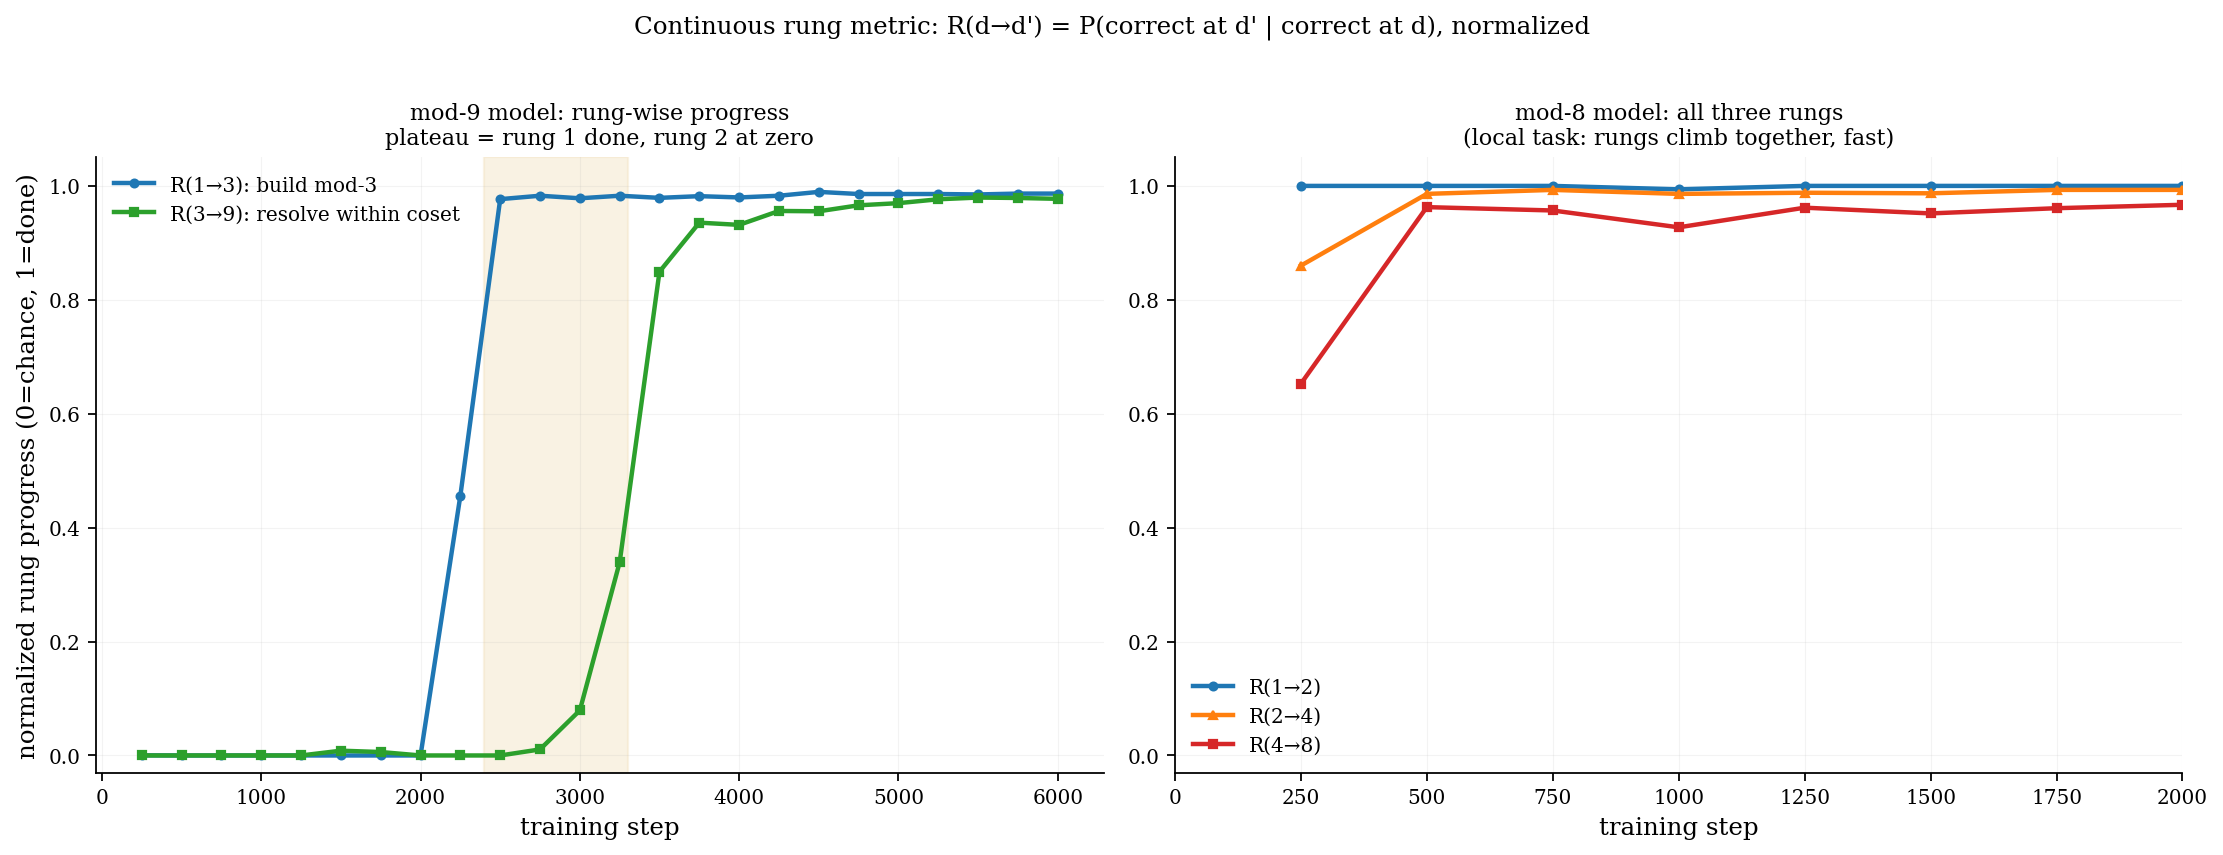
\includegraphics[width=0.8\linewidth]{figs/rung_metric.png}
\caption{\textbf{The rung conditional} $R(d\to d')$: sequential stage structure in both the slow (mod 9) and fast (mod 8) regimes.}
\label{fig:rung}
\end{figure}

\subsection{What changes inside: aggregation and compression}
\label{sec:e1e2}

Two further instruments, specified before the sweep, ran on the same checkpoints (Fig.~\ref{fig:e1e2}).

\textbf{Attention globalizes exactly when the theory says.} For each checkpoint we measure attention mass from the final position onto the numeral's last token vs.\ its earlier tokens (all heads, layers 6--16). In the mod-9 model, cross-token mass jumps from $\sim$2.0 to $\sim$5.3 (summed over heads) precisely in the plateau-onset window (2000--3000; onset 2300 on the behavior curve), with a second rise at the snap. The mod-8 model is the mirror image: a head attends to the last numeral token with weight 1.00 \emph{from step 250 onward at every checkpoint}, and its early-token attention \emph{decays} with training. The same data distribution drives attention in opposite directions, as digit-locality requires.

\textbf{Converged models discard their scaffold.} Why probe for the digit sum at all? It is the human algorithm for this task: mod 8 is read off the last three digits, while mod 9 is computed by summing the digits and reducing the sum---far cheaper than long division. Since mod 9 needs global information and mod 8 does not, we predicted the mod-9 model would build a digit-sum representation at plateau onset, and the mod-8 model would not. The prediction failed: the raw digit sum (e.g.\ $49059 \to 27$) is decodable at $R^2 \approx 0.95$--$0.98$ from every layer already at step 250, \emph{in both models}---the pretrained features carry it (consistent with the pretrained basis, Fig.~\ref{fig:probeextra}). What training does instead is the reverse. As the mod-9 model converges, its \emph{deep} layers (L13--16, the decision site) progressively \emph{discard} the raw sum ($R^2$: $0.98 \to 0.88 \to 0.63 \to 0.56$ at steps 250/2000/3500/6000; best-decoding layer migrates from L14 to L1), with the steepest drop in the plateau-to-snap window---exactly while the mod-9 residue becomes decodable there (Fig.~\ref{fig:probes}a). Early layers retain it; the mod-8 model's curve stays flat. The converged network keeps the residue and deletes the quantity it was computed from. Because a probe shows linear presence, not use (the mod-8 model retains deep-layer $R^2 \approx 0.7$ for a quantity it never needs), the evidential content here is the \emph{within-model change and its timing}---one model deletes, the other does not, on schedule with the behavioral stages. This compression becomes causally relevant in \S\ref{sec:install}.

\begin{figure}[t]
\centering
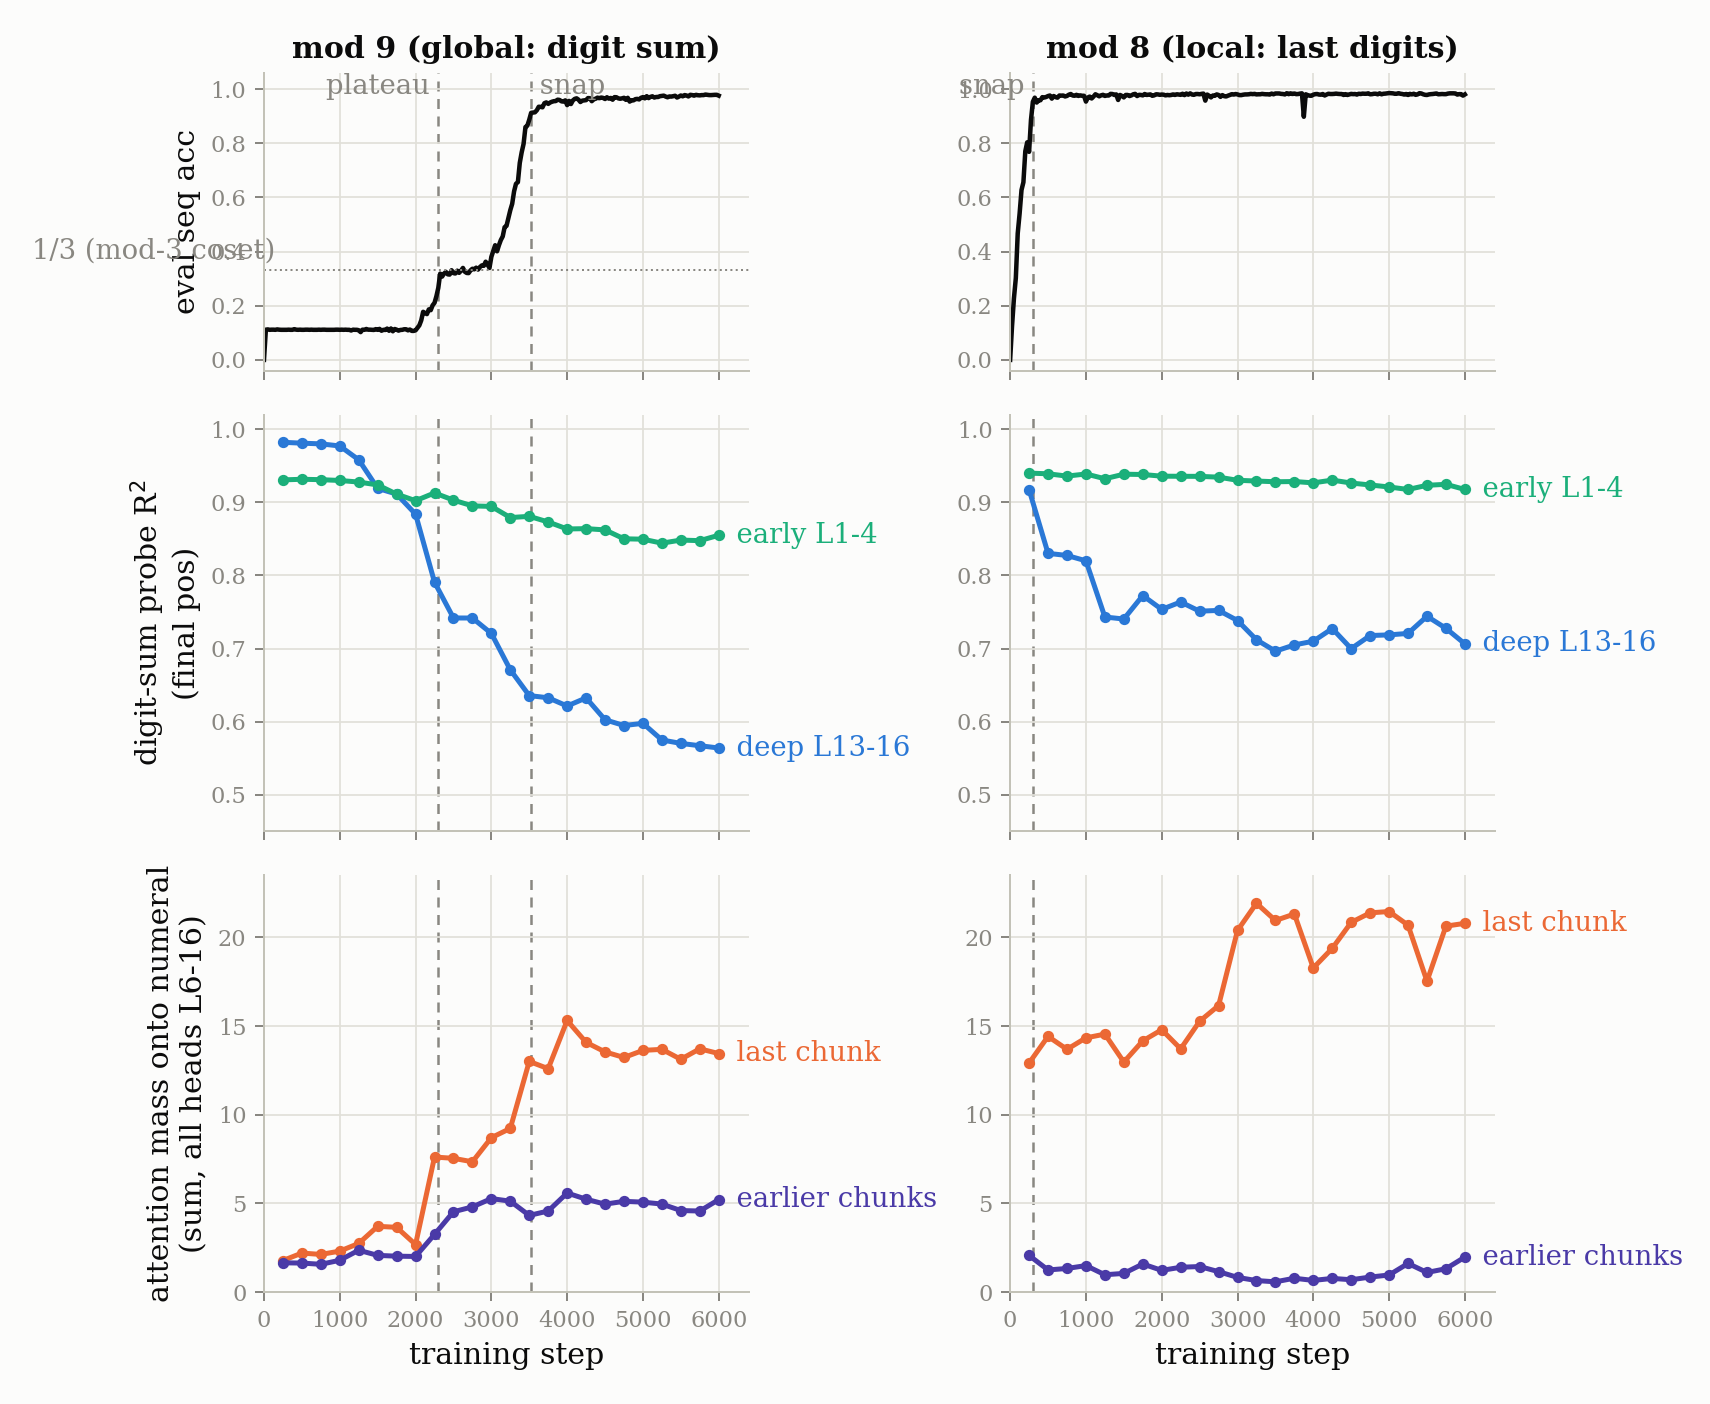
\includegraphics[width=\linewidth]{figs/digitsum_attn_e1e2.png}
\caption{\textbf{Aggregation and compression}. Top: behavior. Middle: raw-digit-sum probe $R^2$ by layer group---the mod-9 model's deep layers discard the raw sum during the plateau$\to$snap window; the mod-8 model never engages it. Bottom: attention from the final position onto numeral tokens---mod-9 globalizes at plateau onset; mod-8 is locked to the last token from step 250. Note absolute mass favors the last numeral token in \emph{both} models (recency, and multi-token numbers are typically summarized at their final token); the discriminating signal is the \emph{trajectory}: mod-9's earlier-token mass triples at plateau onset while mod-8's decays toward zero.}
\label{fig:e1e2}
\end{figure}

\subsection{The account: Fourier readouts composed in order of robustness}
\label{sec:story}

The scorecard, the rung metric, and the aggregation/compression dynamics assemble into one account. Pretraining supplies a \emph{base-10 periodic number basis}: prior static analyses find LM number representations are low-dimensional and Fourier-like with exclusively 2--5-smooth periods $\{2, 5, 10, 25, 50, \dots\}$ \citep{zhou2024fourier,kantamneni2025trig,subspaces2025addition,levy2024digits}---exactly the structure next-token prediction over base-10 text rewards. The base-model probes measure this basis directly in Pythia (parity 0.996, partial mod-8, \emph{no} period-3/9 structure; Fig.~\ref{fig:probeextra}), and the audit (Appendix~\ref{sec:audit}) shows it comes with no modular readouts and no aggregation circuit. Fine-tuning then \emph{composes readouts from this basis in order of noise-robustness}:

\textbf{Local moduli} ($m \mid 10^k$): the needed information already sits in the final numeral token's pretrained features; only a shallow readout is wired $\Rightarrow$ snap, format-irrelevant, attention locked to the last token from the first checkpoints (Fig.~\ref{fig:e1e2}, bottom).

\textbf{Global moduli}: the model must construct (a) an \textbf{aggregation pathway} pooling digit features across all numeral tokens (the attention globalization of \S\ref{sec:e1e2}, arriving at plateau onset) and (b) \textbf{new periodic directions} (period 3, period 9) absent from the pretrained basis. (Appendix~\ref{app:background} gives the background this account presumes---what a periodic feature is, why residues require one, how a period-$T$ plane is estimated and deleted, and why the coarse component is the one greedy descent can use first.) Picture the model's running estimate of the digit sum as a point on a circle. A period-3 readout only needs that point to land in the correct one of three $120^\circ$ wedges; a period-9 readout needs the correct one of nine $40^\circ$ wedges. Early in training the aggregation pathway is half-built, so the estimate wobbles by tens of degrees---too much for $40^\circ$ wedges, tolerable for $120^\circ$ ones. And the tolerant readout alone already halves the loss ($\ln 9 \to \ln 3$: knowing the correct coset is half of everything there is to gain). Gradient descent therefore builds the tolerant, high-reward readout first---locking accuracy at exactly $1/3$ (the plateau)---and the precise one only once the aggregate sharpens (the snap). \emph{The coset staircase is Fourier components arriving in order of robustness}, the natural analogue for our setting of the progress-measure decomposition of grokking \citep{nanda2023progress}. We advance the wedge picture as a model and hold it to a model's standard of evidence: it entails four independent, falsifiable consequences. (i) The spectral components should \emph{arrive} at the behavioral stages---period 3 at plateau onset, period 9 at the snap. (ii) During the plateau, the output logits should carry \emph{only} coset structure. (iii) Removing the coarse component's reward should \emph{invert} the construction order. (iv) The decoded phase's angular error should cross each wedge's tolerance ($60^\circ$, then $20^\circ$) exactly at the corresponding behavioral event. \S\ref{sec:instruments} tests all four.

\begin{figure}[t]
\centering
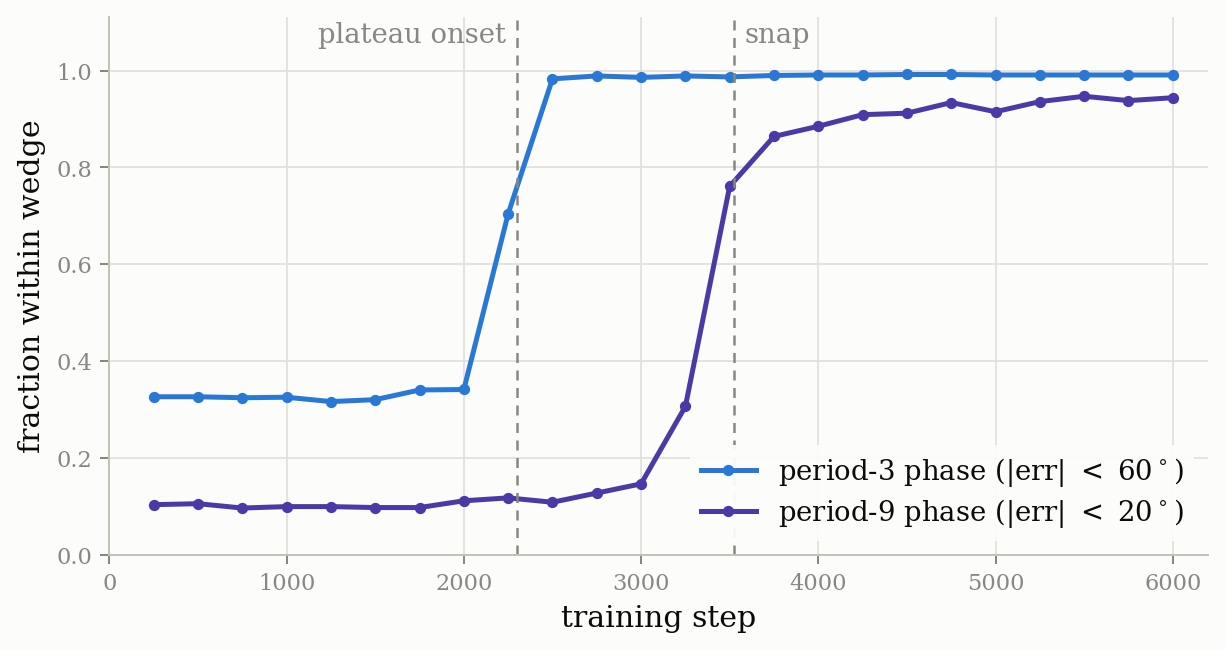
\includegraphics[width=0.8\linewidth]{figs/phase_noise.png}
\caption{\textbf{The wedge account, measured}. Per checkpoint, a ridge decoder is fit to the pair $(\cos, \sin)(2\pi\,\mathrm{ds}/T)$ on training operands (best layer of 13--16); on held-out operands the decoded pair is converted to an angle via atan2 and compared to the true phase. Plotted: the fraction of operands whose angular error is within the class half-width ($60^\circ$ for period 3's $120^\circ$ wedges, $20^\circ$ for period 9's $40^\circ$ wedges). Unlike the categorical probes of Fig.~\ref{fig:probes}, this tests the wedge model in its own units: each phase becomes wedge-accurate precisely at its behavioral stage. Full procedure in Appendix~\ref{app:proc-phase}.}
\label{fig:phasenoise}
\end{figure}


\subsection{The spectra, watched live---and what deletion could not do}
\label{sec:instruments}

Two instruments turn the account into measurements, both run at every checkpoint (plain-language descriptions and exact procedures in Appendix~\ref{app:procedures}): the \textbf{period spectrum} (per layer, how well each candidate periodic feature can be read out, across the local ($N$-)periods and the global (digit-sum) periods; the two families and the identity relating their labels are defined in Appendix~\ref{app:bg-coord}) and the \textbf{output DFT over $Z_9$} (whether the answer logits carry only coset structure or the full residue).

\paragraph{Fourier outcomes.} The period-spectrum sweep confirmed the account's spectral core. In the mod-9 model (layers 13--16), ds-period-3 decodability jumps from $\approx 0$ to 0.96 exactly at plateau onset (steps 2250--2500) and ds-period-9 rises only at the snap (0.77 at 3500, 0.93 after); the $N$-coordinate periods $\{2,5,10,100\}$ are high (0.93--0.95) from the \emph{first} checkpoint---the pretrained basis, present before any task competence---and \emph{decline} to $\approx$0.55 as the model converges, compression now visible in the periodic basis itself. The output-logit DFT over $Z_9$ shows a pure-frequency-3 profile (coset fraction $= 1.000$) for exactly the plateau steps---consequence (ii). And the phase errors cross on schedule---consequence (iv): the fraction of operands within the $60^\circ$ tolerance goes $0.34 \to 0.70 \to 0.98$ across steps 2000--2500 (plateau onset), and within the $20^\circ$ tolerance $0.15 \to 0.76 \to 0.91$ across 3000--4250 (the snap; Fig.~\ref{fig:phasenoise}). The mod-8 control shows no digit-sum-period dynamics at all and \emph{retains} its $N$-periods (0.86--0.95): each model keeps the basis it uses and discards the one it does not. This also settles what ``discarding the scaffold'' (\S\ref{sec:e1e2}) means: what stays decodable at convergence is the pair of periodic components---functions of the residue alone---while what fades is the magnitude information distinguishing sums equal mod 9 (the fade: Fig.~\ref{fig:e1e2}, middle row, $0.98 \to 0.56$; the stay: Fig.~\ref{fig:fourier}, left, ending $0.97/0.93$). How much independent evidential weight each half carries, and the full position-resolved verification, are in Appendix~\ref{app:proc-phase}.

\paragraph{The algorithm, stated.} The converged mod-9 circuit implements per-token rotation accumulation:
\begin{center}
\emph{initialize $\theta = 0$;\quad for each numeral token, rotate $\theta$ by $2\pi\,\mathrm{ds}(\mathrm{tok})/9$;\quad answer $=$ the nearest of the nine digit directions to $\theta$}
\end{center}
(mod 9 this is canonical: since $10 \equiv 1$, updating a running \emph{value} by $v \mapsto 10v{+}d$ and updating a running \emph{digit sum} by $v \mapsto v{+}d$ are the same rotation---no integer total is ever needed). One fact about positions makes the algorithm testable: a causal LM can only store information about tokens it has already read, so if the circuit accumulates token by token, the \emph{intermediate} totals must be present at positions \emph{inside} the numeral. For $N = 49059$, tokenized ``\texttt{ 49}''$\,\cdot\,$``\texttt{059}'', the hidden state above ``\texttt{ 49}'' should encode the running total 13 (as a phase), and the state above ``\texttt{059}'' the full 27. One scope rule: a position covering a \emph{single} token is excluded, because a lone token's digit sum is a function of its identity---even the mod-8 control ``decodes'' it ($R^2 = 0.90$); only the boundary position, where the total spans two tokens, distinguishes accumulation from lookup. With that scope, each clause of the algorithm is separately measured (procedures in Appendix~\ref{app:proc-phase}; Fig.~\ref{fig:phaseswitch}). The \emph{intermediate state} is there: the running total's phase decodes at $R^2 = 0.95$ at the boundary position in the converged mod-9 model, against $-0.27$ in the mod-8 control and negative before the snap. The \emph{update} is the stated rotation: from one numeral token to the next, the decoded angle advances by $2\pi\,\mathrm{ds}(\mathrm{tok})/9$ with median error $4.3^\circ$ at convergence (before the snap: $\approx 90^\circ$, i.e.\ chance; control: chance at every checkpoint). The working variable is \emph{not} an integer count: the alternative---sum first, reduce only at readout---was written down in advance and is ruled out: the count is decodable from step 250 in \emph{both} models (inherited from pretraining, not built for the task) and it fades from the decision site exactly when the phase arrives. There is \emph{no lookahead}: the full total is never decodable at early positions, as causality requires. And the \emph{readout} is nearest-wedge classification: the phase error crosses the $60^\circ$/$20^\circ$ tolerances exactly at plateau onset and snap (Fig.~\ref{fig:phasenoise}), while the output logits carry only coset structure during the plateau. What remains open is the weight-level implementation---\emph{which} heads and MLPs perform the rotation. The algorithm is stated at the level at which the selection law operates, and that level suffices for every intervention in \S\ref{sec:install}.

\begin{figure}[t]
\centering
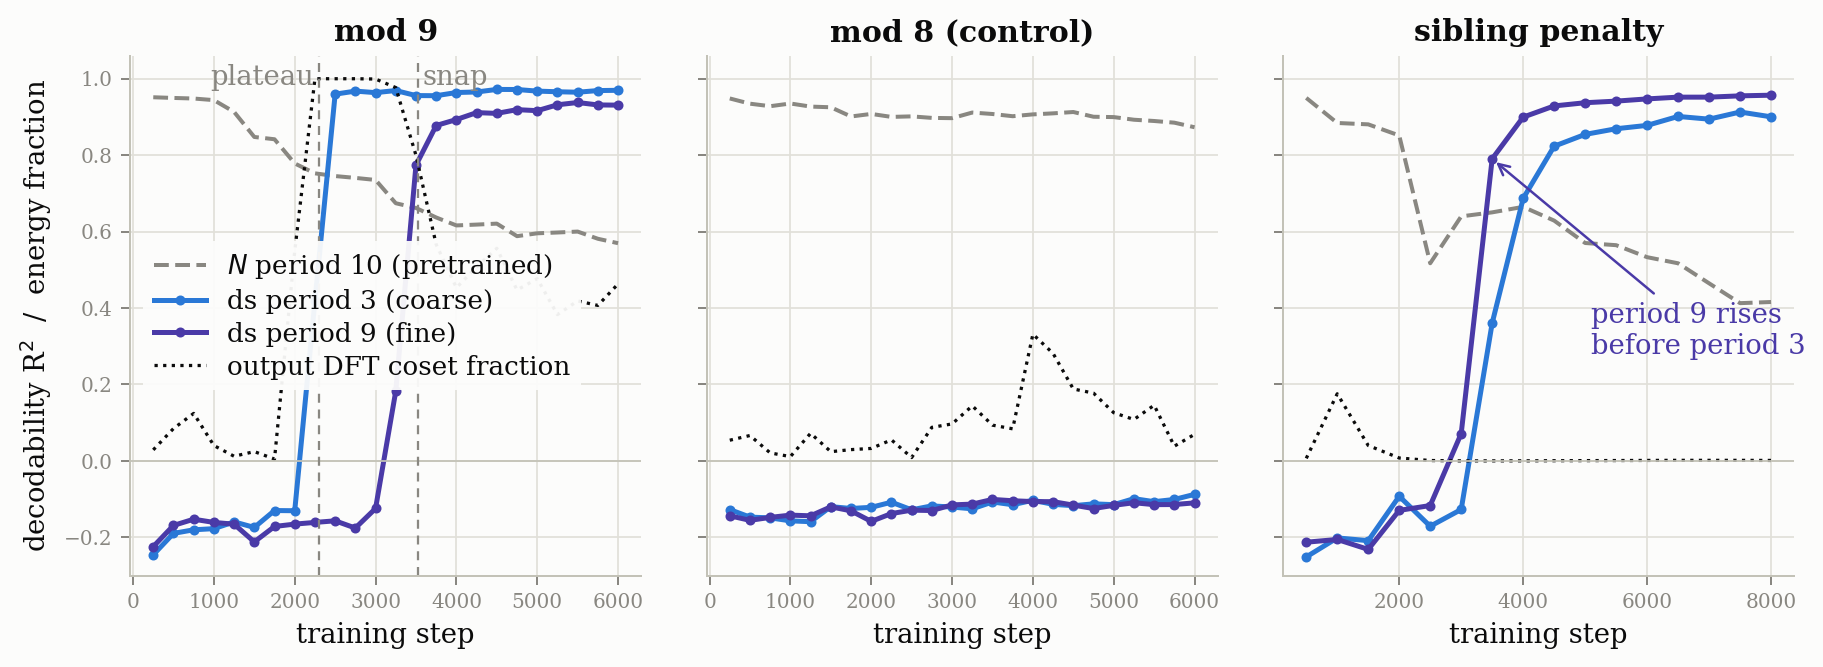
\includegraphics[width=\linewidth]{figs/fourier_dynamics.png}
\caption{\textbf{The spectral construction, watched live}. Left (mod 9): the pretrained value-coordinate basis ($N$, period 10) is present from the first checkpoint and decays; the digit-sum period-3 component arrives exactly at plateau onset and period-9 at the snap; the output-logit DFT (dotted) is pure frequency 3 for precisely the plateau steps. Middle (mod 8): no digit-sum dynamics; the value basis is retained. Right (sibling-penalty run): the coset never forms internally and \emph{period 9 rises before period 3}---construction rerouted, the staircase skipped at a 48\% time cost.}
\label{fig:fourier}
\end{figure}

\paragraph{What deletion could not do.} If the structure above is where the behavior lives, deleting it should break the behavior. We tried three times, each deletion aimed at a specific hypothesis about the carrier. \emph{Class-mean subspaces}: if the decision site holds nine answer clusters, removing the nine cluster-center directions should destroy the readout. \emph{The linear digit-sum direction}: if the readout consults the integer sum, removing its direction should hurt mod 9 and spare mod 8. \emph{The fitted period-3/9 planes themselves}: the code the spectra show existing, removed at L13--16 at every token position. All three left behavior unchanged, with dimension-matched random-subspace controls clean (protocols and numbers in Appendix~\ref{app:procedures}). A cut at other layers, other positions, or higher rank could still land, so the nulls are scoped; what they characterize is the object itself: \textbf{no low-rank, single-site cut we found removes the learned mechanism}---training distributes it redundantly. Site consolidation (\S\ref{sec:scorecard}) is therefore a fact about where the decision is first \emph{readable}, not a causal bottleneck---and the causal case rests on the addition-side interventions of \S\ref{sec:install}, which move behavior in both directions.

\subsection{The base-change test: four predictions, four confirmed}
\label{sec:base9}

The law hinges on ``local vs.\ global \emph{relative to the numeral base}.'' We therefore re-render the operands in base 9: the pile string in the prompt becomes $N$'s base-9 representation (e.g.\ 50000 $\to$ ``75525''), while the label remains $N \bmod m$ computed on the true value. Because base-9 digits are 0--8, prompts are visually indistinguishable from decimal, and the model is never told. This re-derives every prediction, and all four, written before the runs, held (Fig.~\ref{fig:base9}). \textbf{Mod 9 snaps}: the paper's central plateau (f95 $=$ 3725 in base 10) becomes trivial---f95 $=$ \textbf{50}---because $N \bmod 9$ is now the last digit. \textbf{Mod 8 and mod 5 become the strugglers}: base 10's most snap-proof moduli (f95 $\le$ 950) now dwell at chance for thousands of steps and grind---mod 5 reaches criterion at 9000, and mod 8 is still at 0.93 when the 30k budget ends, with no coset plateau above chance. \textbf{Mod 6's plateau height moves}: it plateaus in both bases, but at $0.50$ for $\sim$2500 steps---the predicted $1/2$, since the local factor is now 3 and the resting coset is mod-3---where base 10 rested at $1/3$ (parity). Same modulus, same numbers, same model: which heuristic forms, at what accuracy, and for how long is chosen by the numeral system. No competing account predicts the plateau's height.

\begin{figure}[t]
\centering
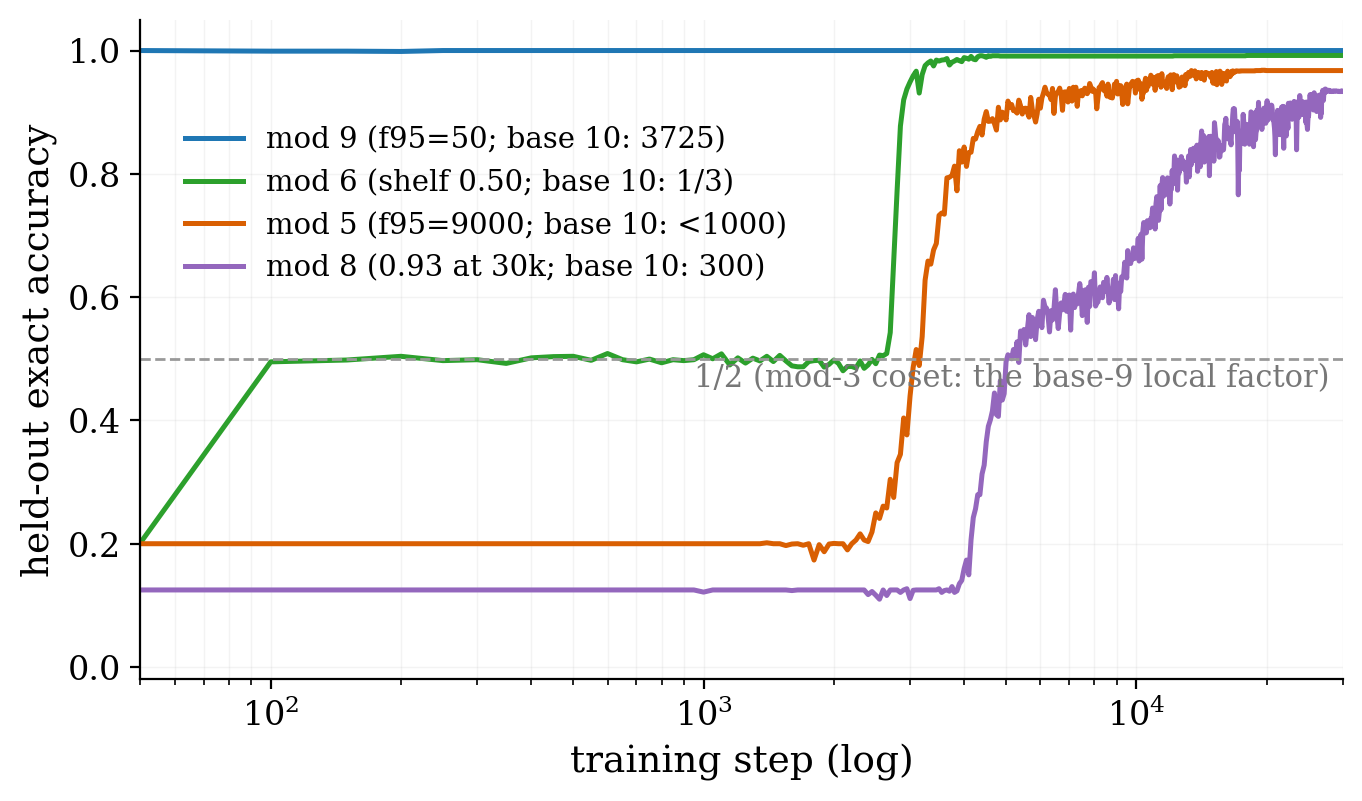
\includegraphics[width=0.72\linewidth]{figs/base9.png}
\caption{\textbf{The base-change test}. The four base-9 runs. Mod 9, base 10's slowest modulus, snaps in 50 steps; mod 5 and mod 8, base 10's fastest, dwell at chance and grind (mod 8 never reaches criterion in budget); mod 6 plateaus at exactly $1/2$---the mod-3 coset, its base-9-local factor---where base 10 plateaued at $1/3$.}
\label{fig:base9}
\end{figure}

\section{How to accelerate past the heuristic---and how not to}
\label{sec:install}

We now intervene. Throughout, a \emph{donor} is a model pre-fine-tuned on a helper task whose weights initialize the target run (in place of base Pythia); all runs share data, schedule, and budget with the from-scratch baseline (f95 $=$ 3725 for mod 9).

\subsection{What fails: installing the coarse answer}

\textbf{The transplant works; the acceleration is refuted.} A converged $N \bmod 3$ donor opens mod-9 training at exactly the plateau (0.332 held-out; a wrong-factor mod-5 donor opens at chance---the transplant is real and factor-specific). But it never helps: across six runs initialized from donor checkpoints of increasing training age (unconverged through overtrained), \emph{no} factor head start beats scratch (f95 5425--7475 vs.\ 3725), the wrong-factor donor ends \emph{better} than the right-factor one, and even the mod-8 control is mildly slowed (generic warm-start friction, \citealp{ash2020warm}). Completing stage $k$ externally does not advance stage $k{+}1$ (Fig.~\ref{fig:round1}, top left; the full checkpoint sweep is in Appendix~\ref{app:dwell}).

\textbf{Entrenchment is invisible to behavior.} At the coset, from-scratch and installed models are indistinguishable---same exact accuracy ($1/3$), same coset agreement ($\approx$0.99), same eval loss---yet from-scratch escapes in $\sim$700 steps where installed models need 2800--4700. Across seeds, installed runs cluster tightly (f95 $\{6250, 6750, 7375\}$) while scratch is fast-but-heavy-tailed ($\{3725, 3800,$ one seed stuck at budget end$\}$): installation trades a stochastic fast escape for a reliably slow one. The same heuristic exists in \emph{escapable} and \emph{entrenched} forms that no behavioral evaluation distinguishes---for the evaluation-gaming reading (\S\ref{sec:related}), the strongest warning in the paper. \emph{Why} installed plateaus are sticky remains open. The obvious suspect---the donor deleted its digit-sum scaffold, so the new task must rebuild it before it can improve---failed its pre-specified test: models escape without ever rebuilding the scaffold (its decodability is flat-to-falling through every escape; Appendix~\ref{app:dwell}). The deletion does track which runs end at a lower \emph{ceiling}, but only as a correlation. The remaining suspects are properties of the loss landscape rather than of the representation, and we leave them to follow-up work.

\subsection{What works: installing the computation underneath}

\textbf{Factors compose (the sign flip).} The \emph{same} mod-3 donor that is 68--98\% slower on mod 9 is \textbf{3$\times$ faster} on mod 6 (f95 200 vs.\ 600), opening at the predicted composite value 0.498 (Fig.~\ref{fig:round1}). The asymmetry is arithmetic before it is anything else. $Z_6 \cong Z_2 \times Z_3$: the mod-6 answer \emph{decomposes} into the pair $(N \bmod 2, N \bmod 3)$, so the donor's computation enters the final solution \emph{unchanged}---it is a coordinate of the answer, already correct on the half of cases where $N \bmod 6 < 3$ (hence the 0.498 start)---and the missing coordinate, parity, is base-local and pretrained (Fig.~\ref{fig:probeextra}), leaving only a readout to wire: exactly the problem class that snaps. $Z_9$, a prime power, does not decompose: mod 3 is a lossy \emph{quotient} of mod 9, no function of the coarse phase recovers the fine one, so the donor contributes nothing to the required construction---and worse, its confident phase-to-digit readout occupies the very pathway the new solution must overwrite, wrong on two-thirds of examples. A factor is a \emph{part} of the answer; a coarsening is a blurry photo of it. Installation has no fixed sign; the sign is computable from divisor structure: \textbf{factors compose, coarsenings entrench}. (Why overwriting costs as much as it does---the $4$--$7\times$ dwell---is the open entrenchment question above.)

\textbf{Scaffolds transfer (the 2$\times$2).} Donors supervised on the \emph{upstream quantities}---the digit sum (which determines mod 9/3, not mod 11) and the alternating sum (mod 11, not mod 9)---were crossed over both targets. Each accelerates only its matched target, massively: digit-sum donor $\to$ mod 9 at f95 $=$ \textbf{200 (18.6$\times$), with no plateau at all} (f25 $=$ 25); alternating-sum donor $\to$ mod 11 at 800 (8.2$\times$); mismatched cells and a format-matched control show only mild generic transfer (1.0--1.5$\times$) (Fig.~\ref{fig:round2}). Notably, supervising the raw digit sum is itself \emph{cheap} (f95 $=$ 1950, half the cost of its own mod-9 coarsening): the expensive thing is never the quantity but reducing it to a residue the pretrained basis lacks. Against the answer-donor's 0.6$\times$, this is the section's law: \textbf{installing the upstream computation is an 18$\times$ accelerant; installing the coarsened answer is an obstruction.}

\textbf{An oracle-injection control prices the readout.} Design: during training, we add to the layer-13 activations (at the answer position) a synthetic vector encoding the \emph{true} phase $(\cos,\sin)(2\pi\,\mathrm{ds}/9)$, computed from the data generator---an oracle the model merely has to learn to \emph{read}. With the oracle present, training reaches ceiling in 25--125 steps: wiring a readout to an existing feature costs $\sim$3\% of from-scratch training, so the 3725-step from-scratch run is almost entirely the wait for the feature to \emph{exist}. The second half of the control: take those trained checkpoints and evaluate them \emph{with the injection turned off}. Every checkpoint scores exact chance (0.110--0.113)---not even the coset formed. With a perfect feature freely available, gradient descent built nothing of its own; a model can sit at ceiling for six thousand steps while acquiring nothing, and no evaluation run with the crutch present can tell. Comparing the three starting conditions---handed the feature itself (25--125 steps), handed the upstream skill as donor weights (200), from scratch (3725)---separates the price of reading a feature, hooking up an inherited one, and building one (Appendix~\ref{app:dwell}).

\textbf{The same law governs curricula.} Scale the task up instead of across: mod 9 on \emph{6-digit} operands is unlearnable from scratch in our budget (chance for 15{,}000 steps). A two-stage curriculum---short operands first, then 6-digit---fixes this, but only in one version. If stage 1 runs to \emph{convergence}, stage 2 opens at 0.534 (the finished circuit already length-generalizes) and reaches criterion in 600 further steps. If stage 1 is stopped \emph{mid-plateau}, stage 2 inherits the coset heuristic and stalls at it (0.66 at 15k) (Fig.~\ref{fig:round2}, right). This is the donor result in curriculum form: hand the next stage a \emph{completed computation} and it composes; hand it the \emph{coarse stage} and it entrenches. (We had guessed the opposite---that transferring \emph{before} convergence would help, the model still being plastic---and the data reversed us.) One law, three appearances: task axis (the sign flip), object axis (computation vs.\ answer), instance axis (curriculum).

\subsection{The staircase is chosen---and it is the fast route}

Removing the coset's loss advantage within-task (penalizing the true answer's two coset siblings, which deletes no information) eliminates the plateau \emph{entirely}, behaviorally and internally---the period spectrum shows the coset stage never forms and \textbf{period-9 rises before period-3}, the order spectral bias always predicted---yet learning is 48--85\% \emph{slower} (f95 5525/6875 vs.\ 3725; Fig.~\ref{fig:round1}, top right). Gradient descent takes the staircase not because it must but because it is the best route available \emph{given nothing but the task's gradient}; every successful acceleration above works by changing what the model is given, never by fighting the stage.

\begin{figure}[t]
\centering
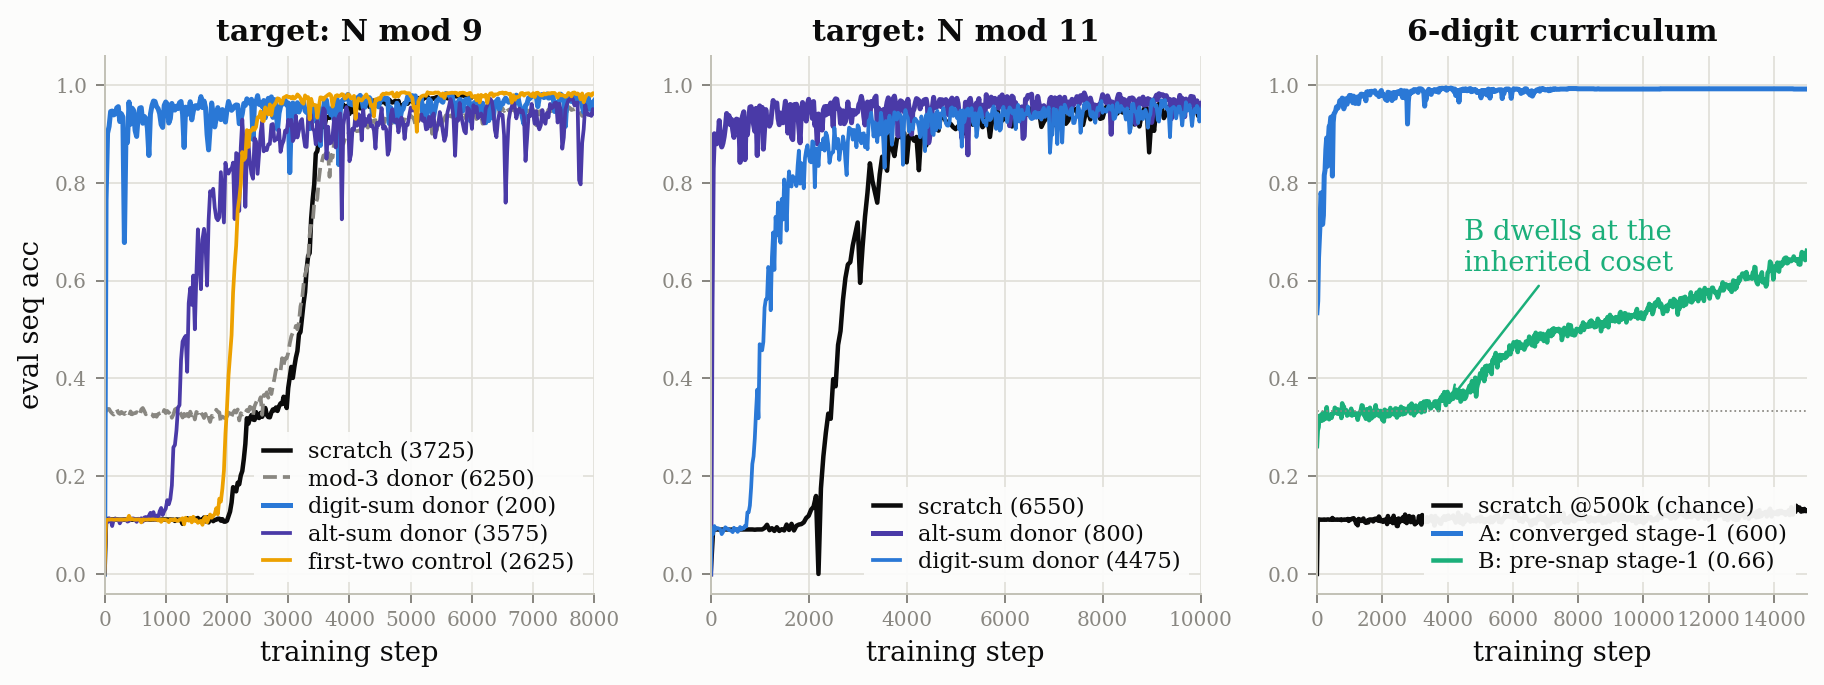
\includegraphics[width=\linewidth]{figs/tx_round2.png}
\caption{\textbf{Round 2}. Left: mod-9 target---the digit-sum (scaffold) donor solves it in 200 steps with no plateau, while the mod-3 (answer) donor is slower than scratch; mismatched/control donors show only mild generic acceleration. Middle: the dissociation mirrored on mod 11. Right: the magnitude curriculum---a converged short-operand stage makes the unlearnable 6-digit task trivial (f95 $=$ 600), while a pre-snap stage donates its coset and entrenches.}
\label{fig:round2}
\end{figure}

\begin{figure}[t]
\centering
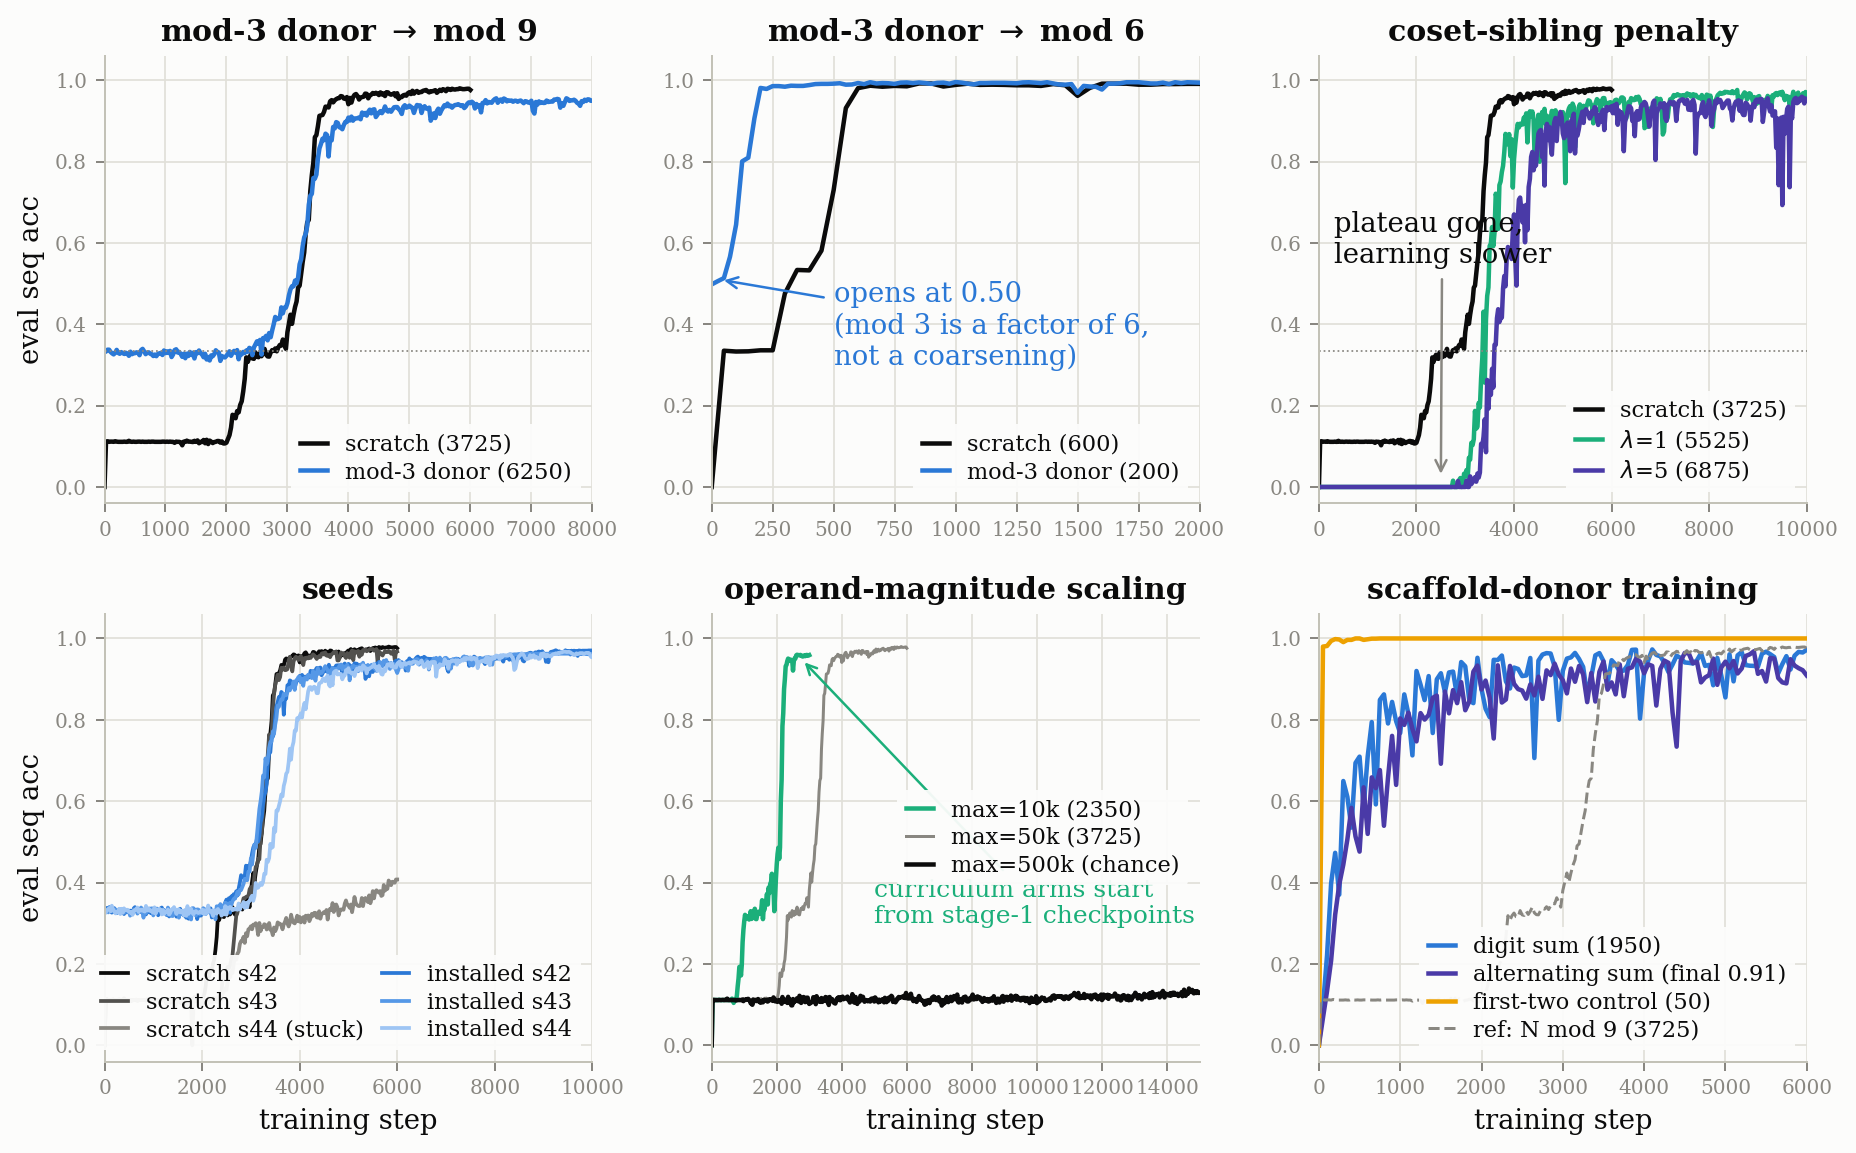
\includegraphics[width=\linewidth]{figs/tx_round1.png}
\caption{\textbf{Round-1 causal batch}. Top: the same mod-3 donor obstructs mod 9 (left) and accelerates mod 6 threefold (middle); removing the coset's loss advantage removes the plateau but slows learning (right). Bottom: seed structure (scratch stochastic, installed uniformly slow); 6-digit operands are unlearnable from scratch in budget while the curriculum stage-1 solves its short-operand slice quickly; supervising raw scaffold quantities is fast.}
\label{fig:round1}
\end{figure}


\section{Related work}
\label{sec:related}

\textbf{Grokking and modular arithmetic.} \citet{power2022grokking,nanda2023progress,gromov2023grokking,zhong2023clock} analyze converged mechanisms for prime-modulus arithmetic over single-token operands in from-scratch transformers. Our central phenomena---digit-locality, coset staging, composition obstruction, pretrained local bases---are structurally impossible in that regime: they require multi-digit tokenized operands and a pretrained substrate. Two works anticipate the \emph{local} half of our law in other settings: \citet{charton2024gcd} finds from-scratch GCD transformers learn products of the base's prime divisors first, and \citet{xu2025principled} show modular addition generalizes out-of-distribution exactly when the modulus divides $10^m$; neither setting produces coset stages, dwell scaling, or fine-tuning dynamics, and neither predicts the global-factor half in advance (plateau heights $d/m$, factor-7 vs factor-3 dwell, prime ramps). \citet{stander2023cosets} find coset structure in converged group-operation networks; we show cosets as \emph{transient, predictable training stages} and manipulate them. \citet{prakash2024finetuning} show fine-tuning enhances an existing circuit in place by comparing endpoint models; our dense-checkpoint site-consolidation result (\S\ref{sec:scorecard}) is the developmental version, watching the in-place upgrade happen.

\textbf{Heuristics in LM arithmetic.} \citet{nikankin2025arithmetic} characterize LM arithmetic as a bag of heuristics at the endpoint of training; we give the heuristics' developmental trajectory, a law for which ones form, and an installation/obstruction toolkit. Static analyses of LM number representations \citep{levy2024digits,zhou2024fourier,kantamneni2025trig,subspaces2025addition} find low-dimensional, Fourier-like, base-10-organized features with 2--5-smooth periods; our base-model probes measure this basis directly in Pythia, and our dynamics show it is the \emph{reason} local moduli snap.

\textbf{Staged learning theory.} The staircase property \citep{abbe2021staircase} and hidden progress in parity learning \citep{barak2022hidden} predict sequential feature acquisition; we exhibit a naturally occurring staircase in a pretrained LM whose stage order is computable from the task (\S\ref{sec:law}) and visible even inside fast transitions (\S\ref{sec:rung}).

\textbf{Warm-starting, transfer, and plasticity.} Warm-started networks generalize worse \citep{ash2020warm}; early training has critical periods \citep{achille2019critical}; continual training loses plasticity \citep{dohare2024plasticity}; extended pretraining makes models more sensitive to fine-tuning damage \citep{springer2025overtrained}. Closest in spirit but opposite in sign, \citet{xu2025groktransfer} \emph{accelerate} grokking by transplanting embeddings from a weaker model. Our installation result is the counterpoint with a mechanism-adjacent twist none of these accounts predict: the transplant is behaviorally perfect yet \emph{never} accelerates, behaviorally identical heuristic states differ severalfold in escape time, the lasting deficit coincides with a measured representational event (scaffold discard at donor convergence), and the timing cost is \emph{worst immediately after convergence}, shrinking with further training.

\textbf{Shortcut learning and evaluation.} Coset heuristics are shortcuts in the sense of \citet{geirhos2020shortcut}---rules that satisfy the training distribution while failing the intended task---but they arise here \emph{without a shortcut opportunity in the data}: our training set is a clean, stratified, operand-disjoint sample of the target rule, containing no spurious cue, no correlated nuisance feature, and no distribution shift at evaluation. The cheap rule is made available by the model's representation, not by the dataset. This sharpens their ``principle of least effort'' into something measurable: with two sub-rules available, the model takes the computationally cheaper one even at a large accuracy cost (mod 14 settles for the parity coset at $1/7$ when the mod-7 coset would pay $1/2$). The installation result (\S\ref{sec:install}) then gives a minimal model of evaluation gaming with exact ground truth: heuristic states that no behavioral evaluation distinguishes differ severalfold in how hard they are to escape.

\section{Conclusion, limitations, and outlook}
\label{sec:limits}

Fine-tuning a pretrained LM on hidden-rule arithmetic follows a law. Which heuristic forms, at what accuracy, and for how long is computable in advance from how the modulus relates to the numeral base, because gradient descent composes readouts from the pretrained periodic basis in order of noise-robustness---the coarse, high-payoff component first. The staircase this produces is chosen, not forced, and it is the fast route given only the task's gradient. The interventions that beat it never fight the stage; they change what the model is given: supply the upstream computation and the plateau never forms ($18.6\times$); install the coarsened answer and it entrenches invisibly ($0.6\times$, undetectable behaviorally). Factors compose, coarsenings entrench---on the task axis, the object axis, and the curriculum axis alike.

\paragraph{Beyond arithmetic.} Nothing in the three findings is arithmetic-specific in kind. Any task with a hidden rule and a cheap coarsening---syntax before semantics, pattern-matching before execution in code models, shortcut policies under RL---has the same structure: a heuristic that captures most of the loss, an optimizer that takes it whenever it is the best gradient bargain, and evaluations that cannot see the difference while the model sits on the plateau. Modular arithmetic is the instance in which the coarsenings are \emph{enumerable} and ground truth is exact, so the selection law, the entrenchment effect, and the computations-not-answers transfer rule can be stated and tested exactly rather than anecdotally. The portable claims are qualitative: heuristics are chosen by computational cost against the model's existing representations; behaviorally identical heuristic states can differ severalfold in how hard they are to escape; and supplying an upstream computation composes where supplying a coarsened answer obstructs. The base-change test (\S\ref{sec:base9}) confirms the within-model form of that portability---re-render the numerals and every prediction moves with the base---and the cross-model sweep (\S\ref{sec:law}) shows both the transfer (five cells, plateau heights exact) and its first boundary (the missing mod-9 staircase).

\paragraph{Limitations.} All deep instrumentation is on one model (Pythia-410m; the behavioral law replicates at 70m and 160m, Fig.~\ref{fig:sizelaw}, but all probes and interventions are 410m-only). The behavioral law now replicates on a second family with a maximally different number tokenizer (Qwen2.5-0.5B, \S\ref{sec:law}): five of six held-out cells with exact plateau heights, and one informative deviation---mod 9 unlearnable from scratch in budget---diagnosed as an aggregation cliff and repaired by the magnitude curriculum (Appendix~\ref{app:lawfigs}). Llama and Gemma families, and mechanism-level replication, remain follow-ups; the instruments travel (the output DFT is vocabulary-independent; the period machinery needs only digit spans). One task domain. Seeds $\times 3$ on the original install comparison but $n{=}1$ on the sign-flip, scaffold-transfer, and base-change headline numbers (replication in progress); deletion-side causal localization returned scoped nulls (\S\ref{sec:instruments}) and finer-grained instruments are deferred. The claim is not that these specific circuits matter in frontier models---it is that this setting yields \emph{predictive, falsifiable} statements about how rule learning proceeds, stalls, and fails in pretrained LMs, at a rigor toy settings have not required of themselves. The installation result adds a practical edge: supplying a curriculum's ``helpful'' intermediate skill can be worse than supplying nothing, and the reason may be measurable in representation space before any fine-tuning begins.

\subsubsection*{Reproducibility statement}
All experiments use a public model family and generated data; generators, trainers (with the boundary guard), probe suites, and per-run metrics will be released. Predictions fixed before the runs are stated in the text alongside their outcomes, including refutations. Dense checkpoints (every 250 steps) for the main runs are retained for re-analysis.

\bibliography{references}
\bibliographystyle{iclr2026_conference}

\appendix

\section{Background: how a network can hold a number}
\label{app:background}

This appendix states, from first principles, the machinery \S\ref{sec:mechanism} uses. Readers familiar with probing and Fourier analyses of LM arithmetic can skip it; \S\ref{app:bg-coord} contains the one methodological choice that is specific to our multi-token setting.

\subsection{Representations, directions, probes, and $R^2$}
\label{app:bg-probe}

At every token position and every layer $\ell$, the model holds a vector $h^{(\ell)} \in \mathbb{R}^{1024}$ (the residual stream; 1024 is Pythia-410m's width). Saying ``feature $y$ is represented at layer $\ell$'' means: there is a direction $w$ such that $w \cdot h^{(\ell)}$ tracks $y$ across inputs. A \emph{probe} is that $w$, found by regression: fit $\hat{y} = w \cdot h + b$ on hidden states from one set of operands, then score it on hidden states from operands never used in fitting.

The score is $R^2 = 1 - \frac{\sum_i (y_i - \hat{y}_i)^2}{\sum_i (y_i - \bar{y})^2}$: the fraction of the target's variance the probe explains. $R^2 = 1$ is perfect prediction; $R^2 = 0$ means the probe does no better than always guessing the mean; \emph{negative} $R^2$ means it does worse than that on held-out data---the honest signature of a feature that is simply not there. This distinction matters for our results: at the first checkpoints, digit-sum-period probes score $R^2 \approx -0.25$ (absent), not $R^2 \approx 0.2$ (weakly present).

Two warnings apply throughout. First, decodability is \emph{presence}, not \emph{use}: a probe can succeed by reading a correlate of the target that the model itself never consults (\S\ref{sec:e1e2} gives the concrete case---the mod-8 model retains a decodable digit sum it demonstrably does not need). Only interventions establish use. Second, absence of decodability is evidence only against \emph{linearly} readable presence at the probed layer and position.

\subsection{Why residues live in periodic features}
\label{app:bg-fourier}

To output $N \bmod 9$, a network needs a quantity that is unchanged when $9$ is added to its input---and no linear function of $N$ has that property (linear functions are monotone; residues are periodic). The natural code is a \emph{circle}: represent a quantity $x$ by the angle $\theta = 2\pi x / T$, i.e.\ by the pair
\[
\big(\cos(2\pi x / T),\; \sin(2\pi x / T)\big),
\]
which is invariant under $x \mapsto x + T$ and therefore carries \emph{exactly} $x \bmod T$ and nothing else. We call the 2-dimensional subspace holding such a pair a \emph{period-$T$ plane}. Two facts make this the code neural networks actually use \citep{nanda2023progress,zhou2024fourier,kantamneni2025trig,subspaces2025addition}: addition becomes rotation (angles add, so a running total can be accumulated by composing rotations, never needing the integer total), and a linear readout of the plane recovers the residue.

Which periods a model has is a question about its training data. Pretraining on base-10 text rewards predicting the next \emph{digit}, and the last digit of $N$ is $N \bmod 10$; so periods $10$ and its divisors $2, 5$ (and coarser magnitude periods like 100) are useful for next-token prediction, while period 3 or 9 is never needed to continue a decimal string. This is the ``2--5-smooth basis'' of prior work, and the base-model probes and first-checkpoint spectra confirm it directly in Pythia: value-coordinate periods $\{2,5,10,100\}$ are decodable at $R^2 \approx 0.95$ \emph{before any fine-tuning}, digit-sum periods $\{3, 9\}$ at $R^2 < 0$.

\subsection{The coordinate choice (what is new in the multi-token regime)}
\label{app:bg-coord}

Prior Fourier analyses of LM arithmetic all restrict operands to \emph{single tokens} (GPT-2: $N \le 520$; Llama-3.1: $N \le 999$), and measure periodicity as a function of the token's numeric value $N$. Our operands span up to six tokens, which changes what the candidate periods \emph{are}. One arithmetic fact governs the labeling and must be stated before the measurement: since $10 \equiv 1 \pmod 9$, $\mathrm{ds}(N) \equiv N \pmod 9$ (casting out nines; likewise mod 3), so for $T \in \{3, 9\}$ ``periodic in the digit sum'' and ``periodic in $N$'' name the \emph{same function} of the operand---the probe target cannot distinguish a circuit that tracks the value's residue from one that accumulates digits. The substantive contrast is therefore not between coordinates for a fixed period but between \emph{kinds of period}: \textbf{local} periods ($T \mid 10^k$: 2, 5, 10, 100), computable from trailing digits and rewarded by next-token prediction, versus \textbf{global} periods (3, 9), which are functions of \emph{all} digits and which pretraining never needs. We fit the same machinery over both families,
\[
x = N,\ T \in \{2, 5, 10, 100\} \quad\text{(the pretrained local basis)}, \qquad x = \mathrm{ds}(N),\ T \in \{3, 9\} \quad\text{(the constructed global periods)},
\]
and the contrast between the \emph{families} is the measurement. We retain the ``ds'' label for the global periods because the accumulation hypothesis (App.~\ref{app:proc-phase}, prefix trace) is about digit-wise construction---but by the identity above the label is interpretive, not observational, and the evidence that the circuit routes through cross-token accumulation comes from the prefix trace, the aggregation dynamics (\S\ref{sec:e1e2}), and the scaffold-donor transfer (\S\ref{sec:install}), never from the probe target itself. (Where the two coordinates \emph{do} genuinely diverge is in the unwrapped quantities---the integer $\mathrm{ds} = 27$ vs.\ the integer $N = 49059$ are different regression targets, which is what licenses the scaffold-fade analysis of \S\ref{sec:e1e2}.) Concretely, for a layer $\ell$, a period $T$ and a coordinate $x$: collect final-position hidden states for 2000 training-pool operands, ridge-regress them onto the two targets $\cos(2\pi x/T)$ and $\sin(2\pi x/T)$, and report the mean held-out $R^2$ of the pair. The two fitted weight vectors, orthonormalized, span the estimated period-$T$ plane---the object the causal test of \S\ref{sec:instruments} deletes.

\subsection{Why the coarse component arrives first}
\label{app:bg-order}

Place the digit sum on a circle. A period-3 readout must separate 3 classes, so its class centers are $120^\circ$ apart; a period-9 readout must separate 9 classes, $40^\circ$ apart. If the model's estimate of the phase carries angular noise---and early in training it must, because the pathway that pools digits across the numeral is still being built---then the coarse readout stays reliable at roughly $3\times$ the noise level that already destroys the fine one. The payoff is also front-loaded: moving from ``uniform over 9 answers'' to ``uniform within the correct coset'' reduces cross-entropy from $\ln 9 = 2.20$ to $\ln 3 = 1.10$ nats, half of the total available reduction, and that half is reachable by the noise-tolerant machinery. Greedy gradient descent thus has a large, immediately realizable gradient toward the period-3 readout and only a small one toward period-9, which is why the coarse component arrives first and the accuracy sits at exactly $1/3$ while it is the only one present.

\paragraph{This is the opposite of spectral bias.} Careful frequency bookkeeping makes the observed order surprising, not expected. On $Z_9$, the \emph{fine} (mod-9) information is carried by the \emph{fundamental}---the lowest frequency, $k=1$, one slow cycle over the nine residues---while the \emph{coarse} (mod-3) information is carried by the $k=3$ harmonic, a wave three times faster. Coarse $\ne$ low-frequency: the coset structure is the \emph{high}-frequency component. Spectral bias \citep{rahaman2019spectral}---networks fit low frequencies first---therefore predicts the fine component before the coarse one. We observe the reverse ($k=3$ arrives $\sim$1200 steps before $k=1$; the output DFT is pure frequency-3 throughout the plateau), because in this setting the ordering is set by payoff per unit of phase precision, not by frequency. The sibling-penalty run completes the argument causally: with the $k=3$ payoff removed, construction proceeds \emph{period-9-first}---the order spectral bias always predicted. The default spectral ordering is real but is \emph{overridden} by the coarse component's payoff asymmetry whenever the objective offers one; delete the payoff and the default reasserts itself.

\section{Exact procedures: output DFT, period planes, projection-ablation}
\label{app:procedures}

Code: \texttt{fourier\_suite.py} (measurements), \texttt{causal\_surgery.py} (interventions). All statistics use 2000 training-pool operands for fitting and 2000 held-out operands for scoring.

\paragraph{Orientation: three instruments, three objects.} Everything in this appendix is one of three measurements, and they look at different things.
\begin{itemize}
\item The \textbf{period spectrum} looks \emph{inside} the network: from the residual-stream activations at one layer (final prompt token), can a linear map read out $\big(\cos(2\pi x/T), \sin(2\pi x/T)\big)$? Notation: ``ds-period-$T$'' means the target is built from the digit sum ($x = \mathrm{ds}(N)$; $T \in \{3,9\}$); ``$N$-period-$T$'' means it is built from the value ($T \in \{2,5,10,100\}$); the number reported is held-out $R^2$. It answers: \emph{which periodic features exist inside the model, and when do they appear?}
\item The \textbf{output DFT} looks at what the model \emph{emits}: the nine answer-digit logits, re-indexed by offset from the true answer and Fourier-transformed. A model that knows only the coset scores the true digit and its two coset siblings equally, which concentrates all the energy at frequency 3. It answers: \emph{does the answer distribution carry only coset structure, or the full residue?} Because it reads the nine answer logits directly, it is independent of vocabulary and tokenization.
\item The \textbf{phase error} converts the period spectrum's planes into degrees: decode the angle from the fitted plane, compare with the true phase, report the fraction of operands within the wedge tolerance ($60^\circ$ for period 3, $20^\circ$ for period 9). It answers: \emph{is the internal angle accurate enough to support the claimed readout?}
\end{itemize}
Presence (spectrum), expression (DFT), and precision (phase error) are three different sentences about the same circuit, which is why all three run at every checkpoint. The remaining item in this appendix, \emph{projection-ablation}, is not a measurement but an intervention: delete a fitted subspace at inference---replace activations by their component orthogonal to it---and ask which behaviors break, against a dimension-matched random-subspace control.

\subsection{Output DFT over $Z_9$ (the coset fraction)}
For each held-out example $i$ with true answer $y_i \in \{0,\dots,8\}$: (1) run the model, take the final-position logits, restrict to the nine digit-token ids: $\ell_i \in \mathbb{R}^9$; (2) center, $\ell_i \leftarrow \ell_i - \mathrm{mean}(\ell_i)$; (3) re-index by \emph{offset from the true answer}, $p_i(\Delta) = \ell_i[(y_i + \Delta) \bmod 9]$, so $\Delta = 0$ is the correct digit and $\Delta = 3, 6$ are its coset siblings; (4) average over examples, $\bar{p}(\Delta) = \mathrm{mean}_i\, p_i(\Delta)$; (5) DFT the 9-point profile, $F_k = \sum_\Delta \bar{p}(\Delta) e^{-2\pi i k \Delta / 9}$ for $k = 0,\dots,4$, and report energies $e_k = |F_k|^2$. The \emph{coset fraction} is $e_3 / (e_1{+}e_2{+}e_3{+}e_4)$. A model that knows only the coset scores logits equally at $\Delta \in \{0,3,6\}$: all non-DC energy at $k=3$, coset fraction $1$ (observed for exactly the plateau checkpoints). A converged model peaks at $\Delta = 0$, spreading energy over all $k$.

\subsection{Period-plane estimation (the decodability spectrum)}
For a layer $\ell$, coordinate $x \in \{N, \mathrm{ds}(N)\}$, and period $T$: (1) collect final-position residual vectors $h_i^{(\ell)} \in \mathbb{R}^{1024}$ for the fit set; (2) form the two targets $t_i = (\cos 2\pi x_i / T,\; \sin 2\pi x_i / T)$; (3) standardize $h$ per dimension and solve the ridge system $W = (H^\top H + \lambda I)^{-1} H^\top t$, $\lambda = 10$, giving $W \in \mathbb{R}^{1024 \times 2}$ (one closed-form solve per layer, batched on GPU); (4) report the held-out $R^2$ of the two predictions, averaged over the cos/sin pair---the ``period-$T$ decodability'' plotted in Fig.~\ref{fig:fourier}; (5) orthonormalize $W$'s columns (QR) to obtain the \emph{period-$T$ plane} $U_T^{(\ell)} \in \mathbb{R}^{1024 \times 2}$, the object interventions operate on. Negative held-out $R^2$ means the feature is absent, not weak.

\subsection{Projection-ablation (deleting a plane at inference)}
Given planes $U^{(\ell)}$ for chosen layers: register a forward hook on \texttt{gpt\_neox.layers[$\ell{-}1$]} (the module whose output \emph{is} \texttt{hidden\_states[$\ell$]}; index 0 is the embeddings) that replaces its output $h$ by $h - U U^\top h$---removing the component of every activation lying in the plane---at all token positions (periodic mode; the earlier class-mean mode projected only the final position, one reason for its null). Conditions: none / target plane(s) / a dimension-matched random plane (QR of a Gaussian matrix). Behavior is then measured on held-out operands as digit-logit argmax: exact accuracy and mod-3 agreement. Ablation at four consecutive layers (13--16) prevents the immediately-downstream layers from re-deriving the deleted phase from the same-position residual; re-import from \emph{other} positions via attention remains possible in principle and is why an ablation null is scoped, not global.

\subsection{Phase-error measurement (Fig.~\ref{fig:phasenoise}) and the prefix trace}
\label{app:proc-phase}

\textbf{Phase error.} For a period $T \in \{3, 9\}$ and a checkpoint: (1) on 2000 training-pool operands, collect final-position hidden states $h^{(\ell)}$ and ridge-fit $W^{(\ell)}$ predicting the two targets $\big(\cos(2\pi\,\mathrm{ds}/T), \sin(2\pi\,\mathrm{ds}/T)\big)$, exactly as in \S\ref{app:bg-coord}; (2) select the layer $\ell^\ast \in \{13,\dots,16\}$ with the best held-out $R^2$; (3) for each of 2000 held-out operands, form the predicted pair $(\hat{c}, \hat{s}) = W^{(\ell^\ast)\top} h^{(\ell^\ast)}$ and decode the angle $\hat{\theta} = \mathrm{atan2}(\hat{s}, \hat{c})$---where the decoded clock hand points ($\mathrm{atan2}$ is the two-argument arctangent: given a point's $(x, y)$ coordinates it returns the point's angle on the full circle, resolving the quadrant ambiguity that $\arctan(y/x)$ cannot); (4) the angular error is $\varepsilon = \hat{\theta} - \theta$ wrapped to $(-180^\circ, 180^\circ]$, with $\theta = 2\pi (\mathrm{ds} \bmod T)/T$ the true phase. A period-$T$ readout partitions the circle into $T$ classes of width $360^\circ/T$, so the decode classifies correctly iff $|\varepsilon| < 180^\circ/T$---the \emph{class half-width}, $60^\circ$ for $T{=}3$ and $20^\circ$ for $T{=}9$. Fig.~\ref{fig:phasenoise} plots the fraction of held-out operands within the half-width, per checkpoint; the wedge model's prediction is that each fraction crosses its threshold at the corresponding behavioral event, which is what is observed. (Where the plane itself is absent---held-out $R^2 < 0$, e.g.\ period 9 before step 3250---the decoded angle is meaningless and the fraction sits at its chance level, $1/T$ of the circle scaled to the half-width: $\approx 0.33$ for $T{=}3$, $\approx 0.11$ for $T{=}9$, exactly the pre-crossing baselines in the figure.)

\textbf{Prefix trace.} Let the numeral occupy token positions $a, \dots, c{-}1$ and let $\mathrm{prefix}_j$ be the digit sum of tokens $a..j$ (for $N = 49059$ tokenized as ``\texttt{ 49}'',``\texttt{059}'': $\mathrm{prefix}_0 = 13$, $\mathrm{prefix}_1 = 27$). By the identity of App.~\ref{app:bg-coord} the prefix digit sum and the prefix \emph{value} are congruent mod 9, so the probe target is the running \emph{residue} phase however the model computes it; the cell tests cross-token accumulation, not a digit-sum-versus-value route---a distinction that is empty mod 9. At each within-numeral position $j$ we probe the hidden state \emph{at that position} for two targets: the \emph{prefix} phase $(\cos,\sin)(2\pi\,\mathrm{prefix}_j/9)$ and the \emph{full}-sum phase, fit on training operands and scored held-out as above. Interpretation rule fixed in advance of reading the numbers: a single-token position's prefix is a deterministic function of that token's identity, so decodability there is expected of \emph{any} model (the mod-8 control confirms this at $R^2 = 0.90$) and is excluded; only \emph{cross-token} positions, where the target requires combining digits across tokens, bear on accumulation. The reported cells are: cross-token prefix phase $0.95$ (converged mod-9) vs.\ $-0.27$ (mod-8) vs.\ negative (mod-9 pre-snap), and full-sum phase at early positions negative everywhere (no anticipation).

\textbf{Transition rule (the increment test).} The prefix trace verifies the accumulator's \emph{states}; a second, dense-checkpoint sweep verifies its \emph{update}. For each held-out operand, decode the phase at consecutive numeral positions $j, j{+}1$ (best layer of 13--16, fit as above) and form the increment $\Delta\hat{\theta} = \hat{\theta}_{j+1} - \hat{\theta}_j$; per-digit rotation predicts $\Delta\theta = 2\pi\,\mathrm{ds}(\mathrm{tok}_{j+1})/9$, the digit sum of the newly read token. Converged mod-9: median increment error $4.3^\circ$, fraction within $20^\circ$ $= 0.95$. Before the snap: chance (median $\approx 90^\circ$, fraction $0.10 \approx 20/180$). Mod-8 control: chance at every checkpoint. Rule and states arrive together---cross-token phase $R^2$ goes $-0.25 \to 0.19 \to 0.78 \to 0.89$ across steps 3000/3250/3500/3750, precisely the snap window, co-timed with the final-position period-9 arrival of Fig.~\ref{fig:fourier}. The same sweep rules out an alternative fixed in advance, a \emph{count-then-wrap} intermediate stage (aggregate the integer sum, wrap only at readout): the cross-token \emph{count} is decodable from step 250 in the mod-9 model \emph{and} the mod-8 control alike ($0.98$ vs.\ $0.94$---the pretrained, magnitude-confounded feature of \S\ref{sec:e1e2}, not a constructed intermediate), never leads the phase in any task-specific sense, and its deep-layer (L13--16) readout falls $0.98 \to 0.78$ with the steepest drop across the snap itself, while its best-decoding layer migrates from L20--24 to L2--6. The decision site exchanges the count for the phase at the moment the rotation circuit arrives: the scaffold was inherited, never wrapped, and evicted on the arrival of the mechanism that replaces it (Fig.~\ref{fig:phaseswitch}). (Scope: period-9 targets only---the analogous question for the coset stage's period-3 machinery is untested; and 2-token numerals afford a single increment step.)

\begin{figure}[t]
\centering
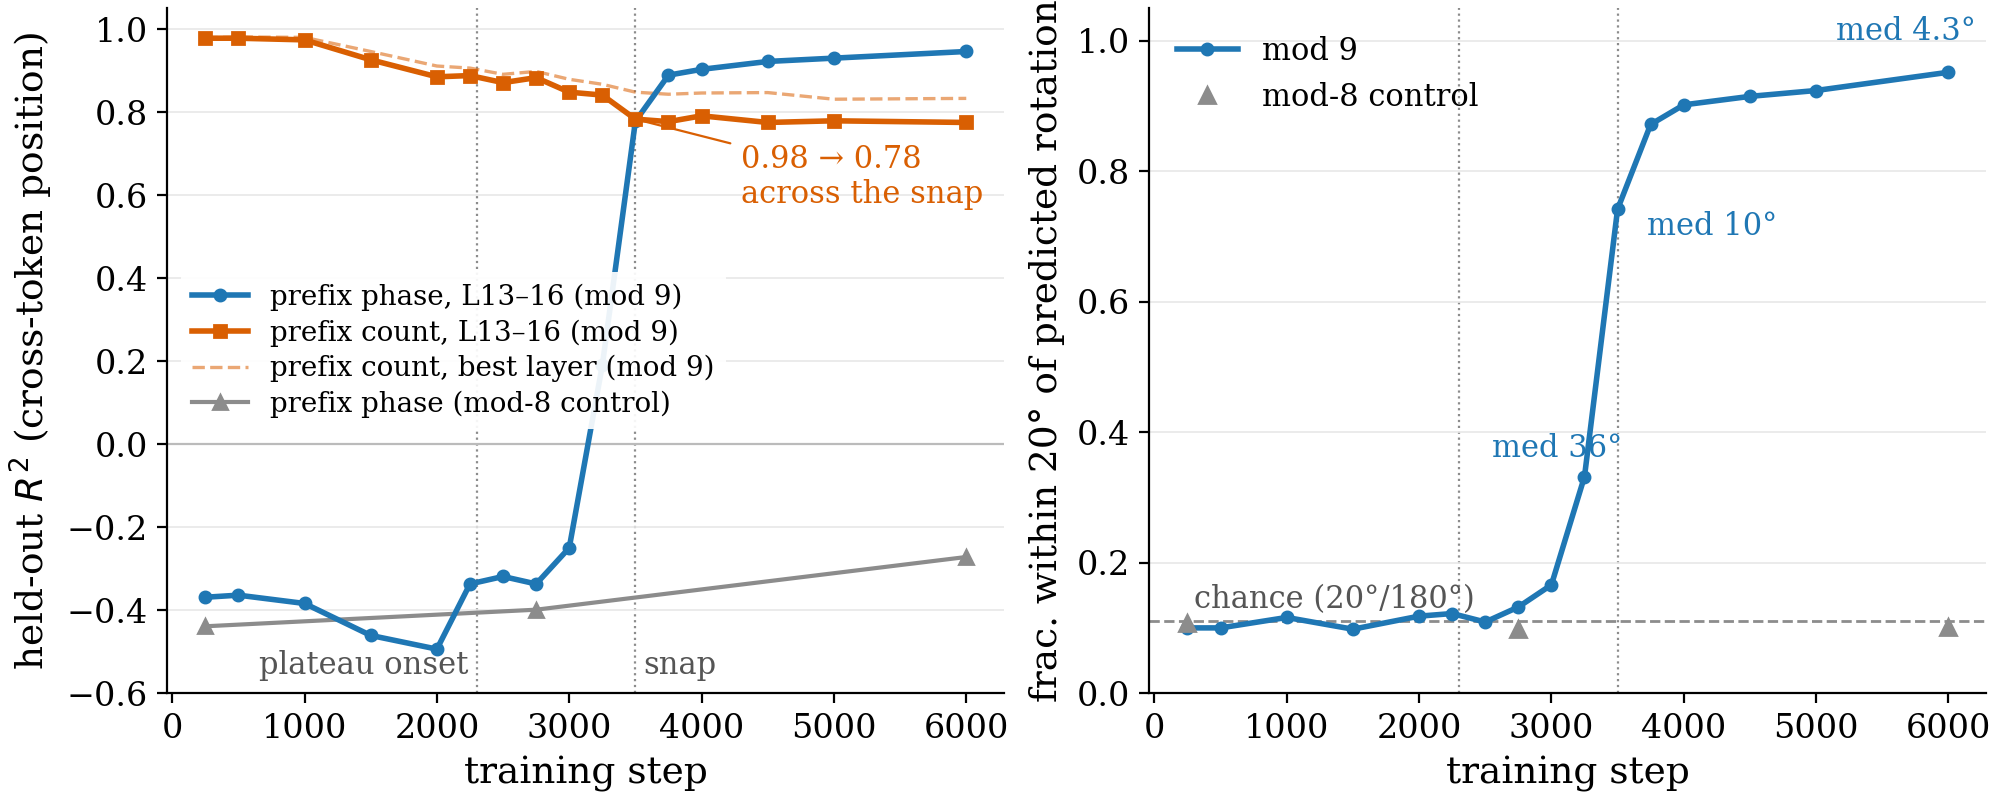
\includegraphics[width=\linewidth]{figs/phase_switch.png}
\caption{\textbf{The mechanism-switch test}. Left: at the cross-token position, the prefix-\emph{phase} readout (L13--16) arrives in the snap window while the prefix-\emph{count} readout is evicted from the same layers---its steepest drop is across the snap itself---and the count's all-layer best (dashed) stays high because early layers retain it; the mod-8 control never acquires the phase. Right: the transition rule, measured---the fraction of per-token phase increments within $20^\circ$ of the predicted rotation $2\pi\,\mathrm{ds}(\mathrm{tok})/9$ rises from exact chance ($20/180$) to $0.95$ at the snap; median errors annotated; the control sits at chance at every checkpoint. The count-then-wrap alternative, fixed in advance, is ruled out by the left panel: the count predates the task (present in the control), fades rather than leads, and the rotation circuit arrives whole.}
\label{fig:phaseswitch}
\end{figure}

\paragraph{Scoping: what the probe targets can and cannot show.} Two cautions bound the readings above. First, by the identity of App.~\ref{app:bg-coord}, the period-$\{3,9\}$ targets are the same functions of the operand whether labeled by digit sum or by value, so no period probe can, by itself, show that the circuit routes through digit-wise accumulation---that claim rests on the position-resolved cells of this section (prefix trace, increments) and the aggregation dynamics (\S\ref{sec:e1e2}). Second, the phase pair is a function of the answer, so its decodability at the consolidated decision site \emph{at convergence} is close to entailed by behavioral accuracy plus the (observational) site consolidation of \S\ref{sec:scorecard}; the endpoint value of the ``stays'' half of \S\ref{sec:instruments} accordingly carries little independent weight. The independent content lies in the \emph{fade}, which no amount of task success requires; in the sibling-penalty run, where behavior is a featureless ramp while the spectra expose fine-first construction (Fig.~\ref{fig:fourier}, right); and in two dissociations showing the probe and the behavior are different measurements---the digit-sum donor holds a ds-period-9 plane at $R^2 \ge 0.95$ with no mod-9 behavior at all, and the oracle-injection model sits at ceiling owning nothing (App.~\ref{app:dwell}).

\section{Layer-by-layer views: the converged lens ladder and the base-model probes}
\label{app:scorecard}

Fig.~\ref{fig:probeextra} shows two results from \S\ref{sec:scorecard} resolved by layer rather than by training step. Left: in the converged mod-8 model the local decision materializes at L12--14, with only a soft $2{<}4{<}8$ ordering inside---site consolidation rather than a clean depth ladder. Right: the base-model probes that refuted our own written-in-advance prediction that no residue would be decodable before fine-tuning: parity at 0.996 and mod-8 partial, mod-3/9 at chance---the pretrained local basis. Its converse is equally diagnostic: the mod-8 probe applied to the \emph{mod-9} model reads a flat 0.5--0.59 at every checkpoint---the pretrained parity/mod-4 content, present regardless of task---and the rest of the mod-8 feature is never built. Nothing needed is missing from the start; nothing unneeded is ever added.

\begin{figure}[h]
\centering
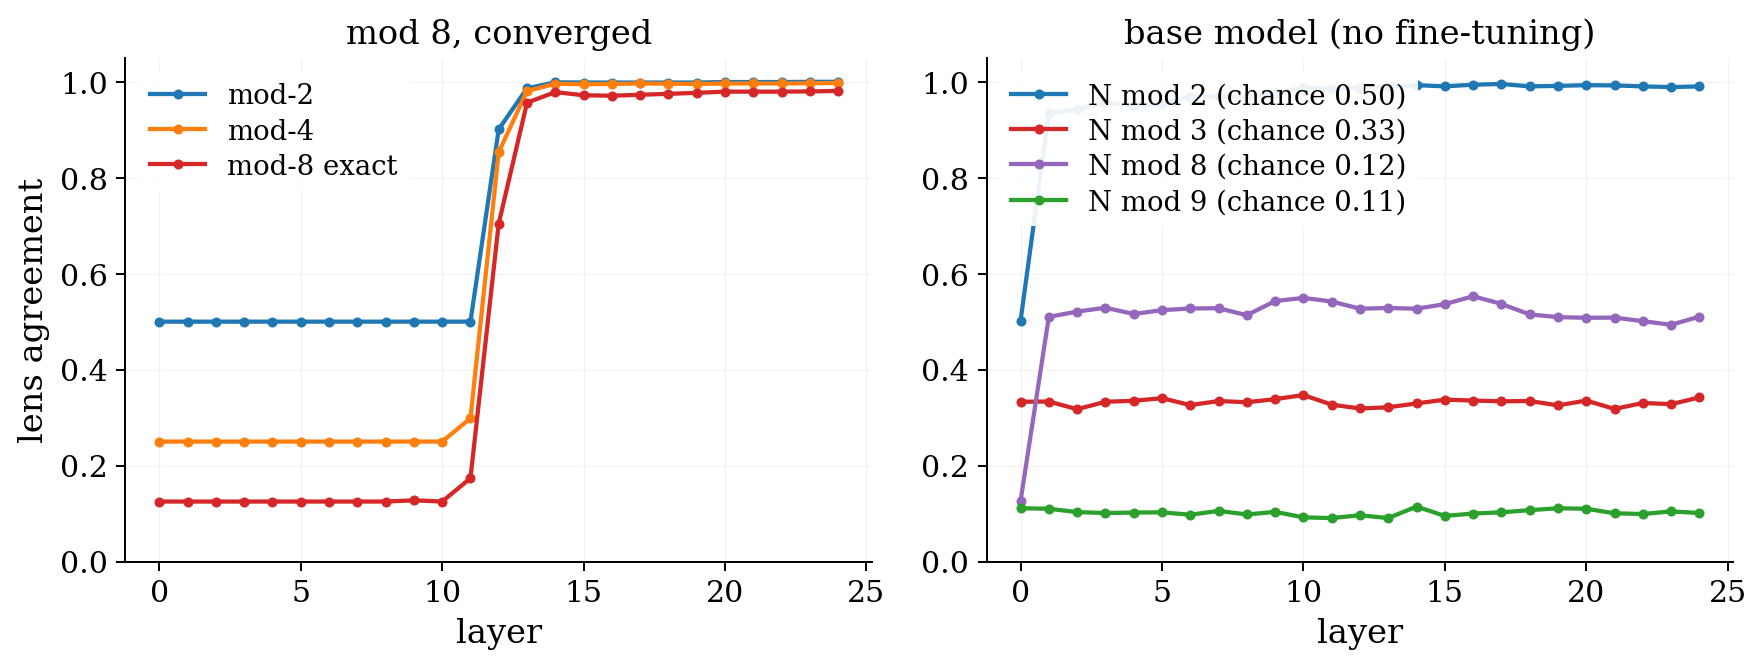
\includegraphics[width=\linewidth]{figs/probe_depth_extra.png}
\caption{Layer-by-layer views accompanying Fig.~\ref{fig:probes}b. Left: the converged mod-8 lens ladder---the local decision materializes at L12--14 with a soft $2{<}4{<}8$ ordering inside. Right: base-model probes per layer---parity at 0.996 and mod-8 partial, with mod-3/9 at chance: the pretrained local basis.}
\label{fig:probeextra}
\end{figure}


\section{Base-model audit and the format sweep}
\label{sec:audit}

\paragraph{Base-model audit.} Zero-shot and $\{4,8,16\}$-shot evaluation of base Pythia-410m across four formats (\texttt{mod}, \texttt{\%}, \texttt{remainder}, \texttt{nimsimple}) $\times$ moduli 2--10 $\times$ operand magnitudes 1--5 digits: above one digit, exact accuracy is at chance \emph{everywhere}, including parity (0.53 vs.\ 0.50 chance) and including the code-native \texttt{\%} operator. The only competence is one-digit copying ($n \bmod m = n$ for $n<m$). There is no latent modular \emph{behavior} to elicit (though \S\ref{sec:mechanism} shows there are latent \emph{features}).

\paragraph{Format is second-order.} Fine-tuning speed to f95 on five-digit operands, identical held-out pools across cells (Table~\ref{tab:formats}). A prompt that is just the number, a prompt about assigning items to counters, and a prompt that actively \emph{lies} about the modulus all land in the same band as explicit \texttt{"N mod 9 ="}---the misleading rule is in fact slightly faster than the truthful one (4975 vs.\ 5200) and shows no early contamination toward the implied modulus. The ``mod'' token confers no advantage, consistent with the audit: there is nothing for it to unlock. Supervision is everything; the task description is decoration. Format does modulate the \emph{duration} of intermediate plateaus (mod-3 dwell 900--2950 steps across cells)---second-order friction---but never the structure of the trajectory.

\begin{table}[h]
\centering
\small
\begin{tabular}{lcc|lcc}
\toprule
cell & mod 8 & mod 9 & cell & mod 8 & mod 9 \\
\midrule
puremod    & 350 & 5200 & bare       & 325 & 3275 \\
modplus1   & 350 & 5550 & unrelated  & 375 & 6075 \\
remainder  & 325 & 3050 & conflict   & 275 & 4975 \\
leftover   & 275 & 8150 & nimsimple  & 300 & 3800 \\
\bottomrule
\end{tabular}
\caption{f95 (steps) across eight formats. The spread across \emph{formats} ($\le 2.7\times$) is small against the spread across \emph{moduli} (15--25$\times$). \texttt{bare} is just the numeral; \texttt{unrelated} describes a nonsense assignment; \texttt{conflict} states the \emph{wrong} rule.}
\label{tab:formats}
\end{table}

\section{The law in more detail}
\label{app:lawfigs}

Fig.~\ref{fig:moremods} shows the moduli 10--16 sweep behind the six held-out-moduli confirmations; Fig.~\ref{fig:magsize} shows how plateau dwell scales with operand magnitude and model size. The two replication sweeps summarized in \S\ref{sec:law} follow in full.

\paragraph{Cross-model replication.} The predictions---trajectory class and plateau height only, since f95 is not comparable across architectures---were fixed in advance for six cells and run on Qwen2.5-0.5B, whose tokenizer splits numbers into single digits, the maximally different segmentation from GPT-NeoX's multi-digit chunks (Fig.~\ref{fig:qwen}). Five of six confirmed: mod 8 and mod 10 snap (f95 $=$ 100 and 50); mod 6 plateaus at $0.33$ for 2400 steps; mod 14 plateaus at $0.143$ for 6500 steps and then climbs \emph{through a second, transient plateau at $0.50$---the mod-7 coset, the divisor staircase's next rung, visible behaviorally}; mod 11 rises with no plateau at any divisor value. The sixth cell failed, informatively: mod 9 never leaves chance in the 25k budget---no coset stage, no snap. The local/global split survives (the global cell became \emph{harder}, not easier); what does not transfer unconditionally is the staircase itself: under digit-level tokenization, the coset stage Pythia builds by step 2300 did not form at all. Follow-up runs resolve the deviation. \emph{Diagnosis}: the failure is a position cliff. Mod 9 over 3-token operands (max 999) learns in 300 steps---with \emph{no} coset plateau---while 4-token operands (max 9999) sit at chance for 5000 steps; and the converged endpoint of the failed 5-token run carries no trace of the periodic features (ds-period-3/9 held-out $R^2 \le -0.001$ at every layer, no output-DFT structure): a true optimization equilibrium, not hidden progress. The successful mod-6 cell, probed identically, holds its global-factor plane at $R^2 = 0.998$---the feature exists exactly where it was needed and reachable. \emph{Repair}: initializing the failed cell from the converged 3-token stage (the magnitude curriculum of \S\ref{sec:install}) opens above chance zero-shot (0.234) and reaches criterion in 575 steps; the intermediate 4-token rung opens at 0.495 and completes in 175. Both rescues are again plateau-free. The reading: where aggregation improves \emph{gradually} (Pythia), a noisy intermediate regime exists in which the coarse readout pays, and the staircase forms; where aggregation is all-or-nothing (digit tokenization's position cliff), no such regime exists and construction is fine-first. The ordering \emph{principle}---loss reduction per unit of precision, given the basis---is what transfers; the ordering itself is not required to.

\paragraph{Scale replication.} The same template run \emph{down} the Pythia family---70m and 160m, five cells each over moduli $\{6, 8, 10, 11, 14\}$, predictions fixed in advance---confirms all ten cells (Fig.~\ref{fig:sizelaw}): mod 10 snaps at both sizes (the discriminating case again), mod 6 rests at exactly $1/3$ and mod 14 at exactly $1/7$ before climbing, and mod 11 ramps with no divisor plateau. Mod 14 prefers the $1/7$ parity coset to the available $1/2$ at every scale tested: the cost-over-accuracy selection is a property of the representation, not of capacity. Capacity moves only the \emph{clock}---never the trajectory class or the plateau height---in two measured ways. On mod 6, size trades against operand magnitude: 70m at max operand $5\times10^4$ dwells about as long as 410m at $5\times10^5$ (Fig.~\ref{fig:magsize}). On mod 14 at matched magnitude, dwell lengthens only moderately at 70m/160m ($\sim$2000 vs.\ 1500 steps at 410m), with most of the size cost falling in the post-plateau climb instead (f95 2800 at 410m vs.\ 15500--17500)---capacity matters most for the \emph{fine} stage, consistent with the precision account of \S\ref{sec:mechanism}.

\begin{figure}[h]
\centering
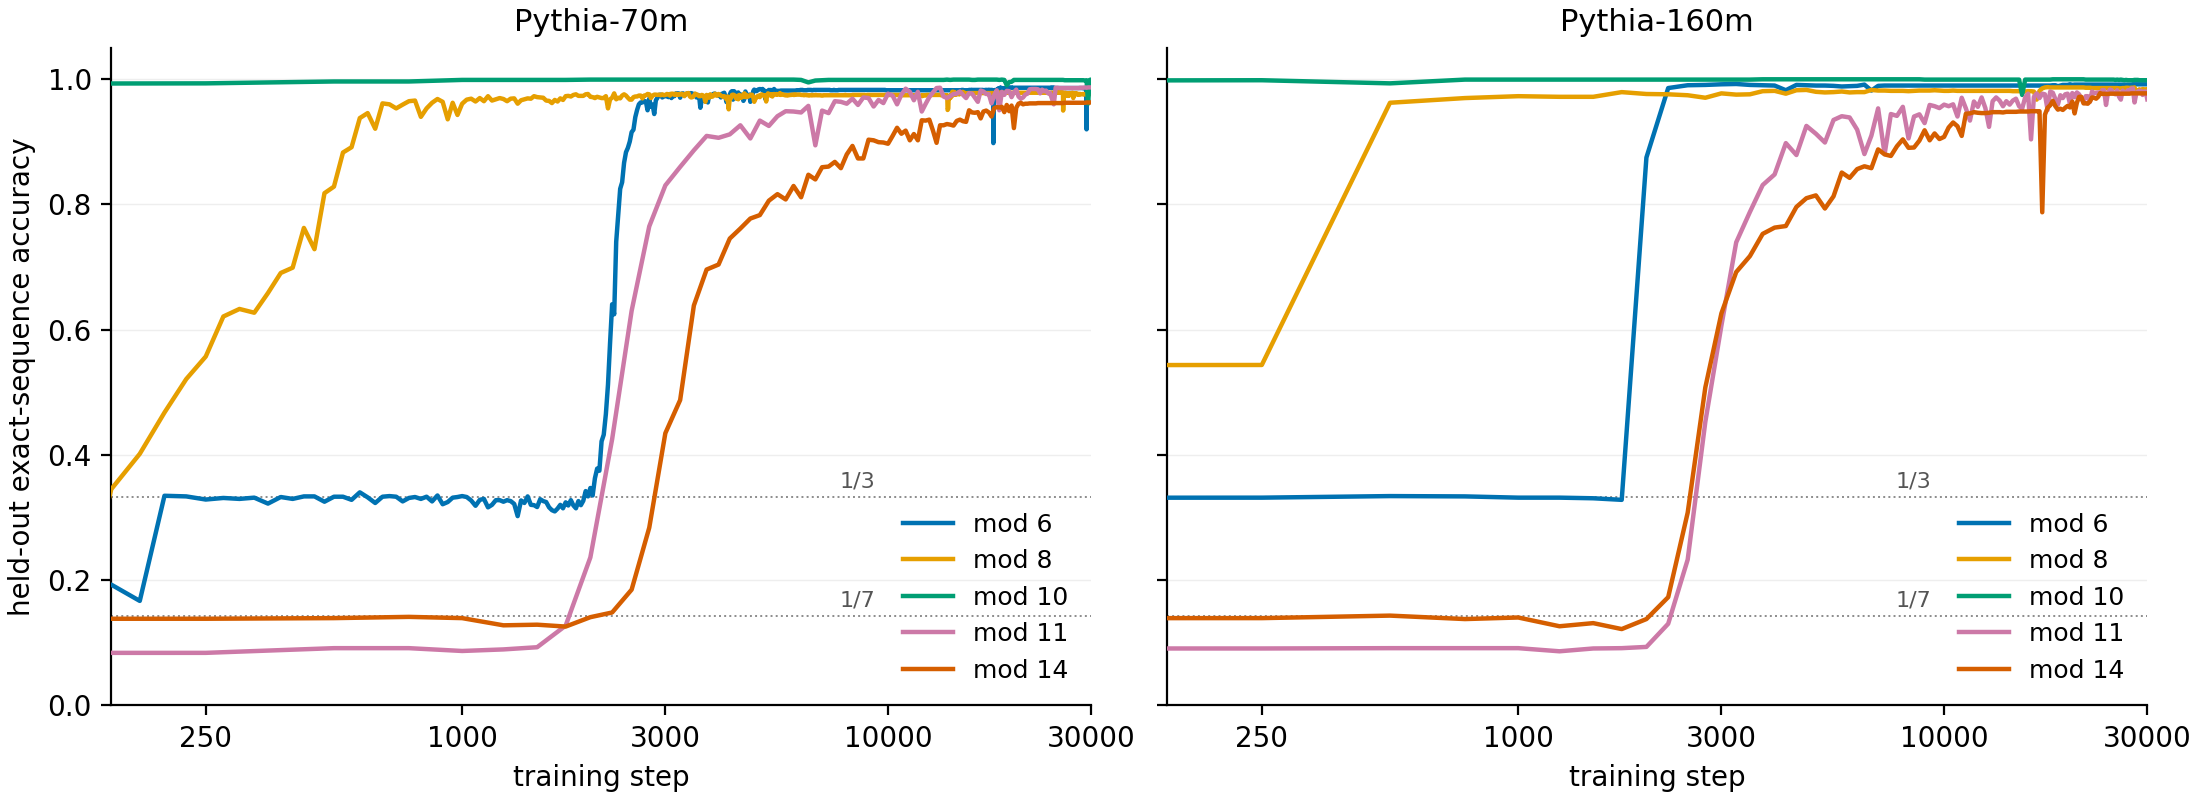
\includegraphics[width=\linewidth]{figs/sizelaw.png}
\caption{\textbf{Scale replication (Pythia-70m and 160m)}. Five cells per size, one seed; log-scaled step axis: mod 8 and mod 10 snap; mod 6 plateaus at exactly $1/3$ and mod 14 at exactly $1/7$ (dotted lines) before climbing; mod 11 ramps with no divisor plateau.}
\label{fig:sizelaw}
\end{figure}

\begin{figure}[h]
\centering
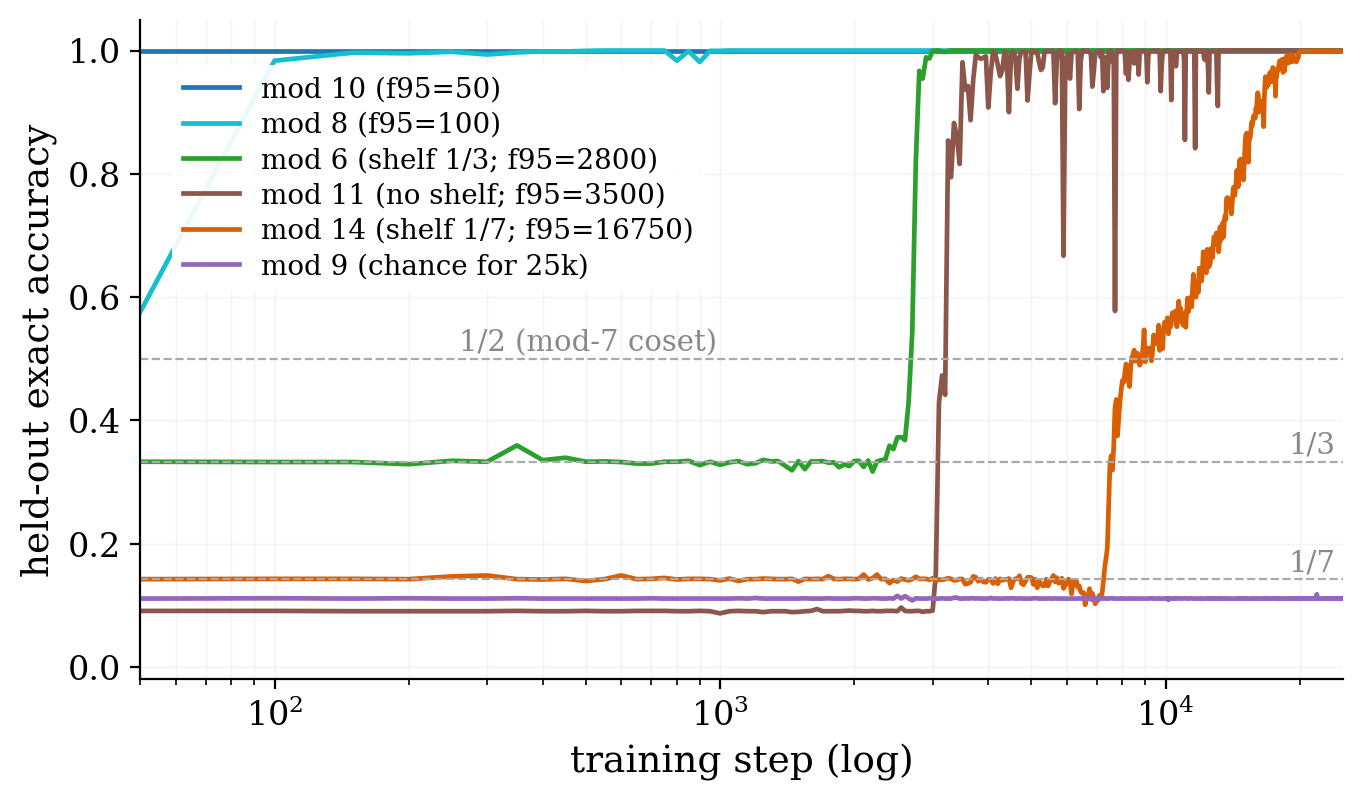
\includegraphics[width=0.72\linewidth]{figs/qwen_law.png}
\caption{\textbf{Cross-model replication (Qwen2.5-0.5B)}. Six held-out cells, one seed: local moduli snap; mod 6 and mod 14 plateau at exactly $1/3$ and $1/7$; mod 14 climbs through a transient second rung at the mod-7 coset ($1/2$); mod 11 shows no divisor plateau. The deviation: mod 9 stays at chance for the full budget---the staircase itself did not form under digit-level tokenization.}
\label{fig:qwen}
\end{figure}

\begin{figure}[h]
\centering
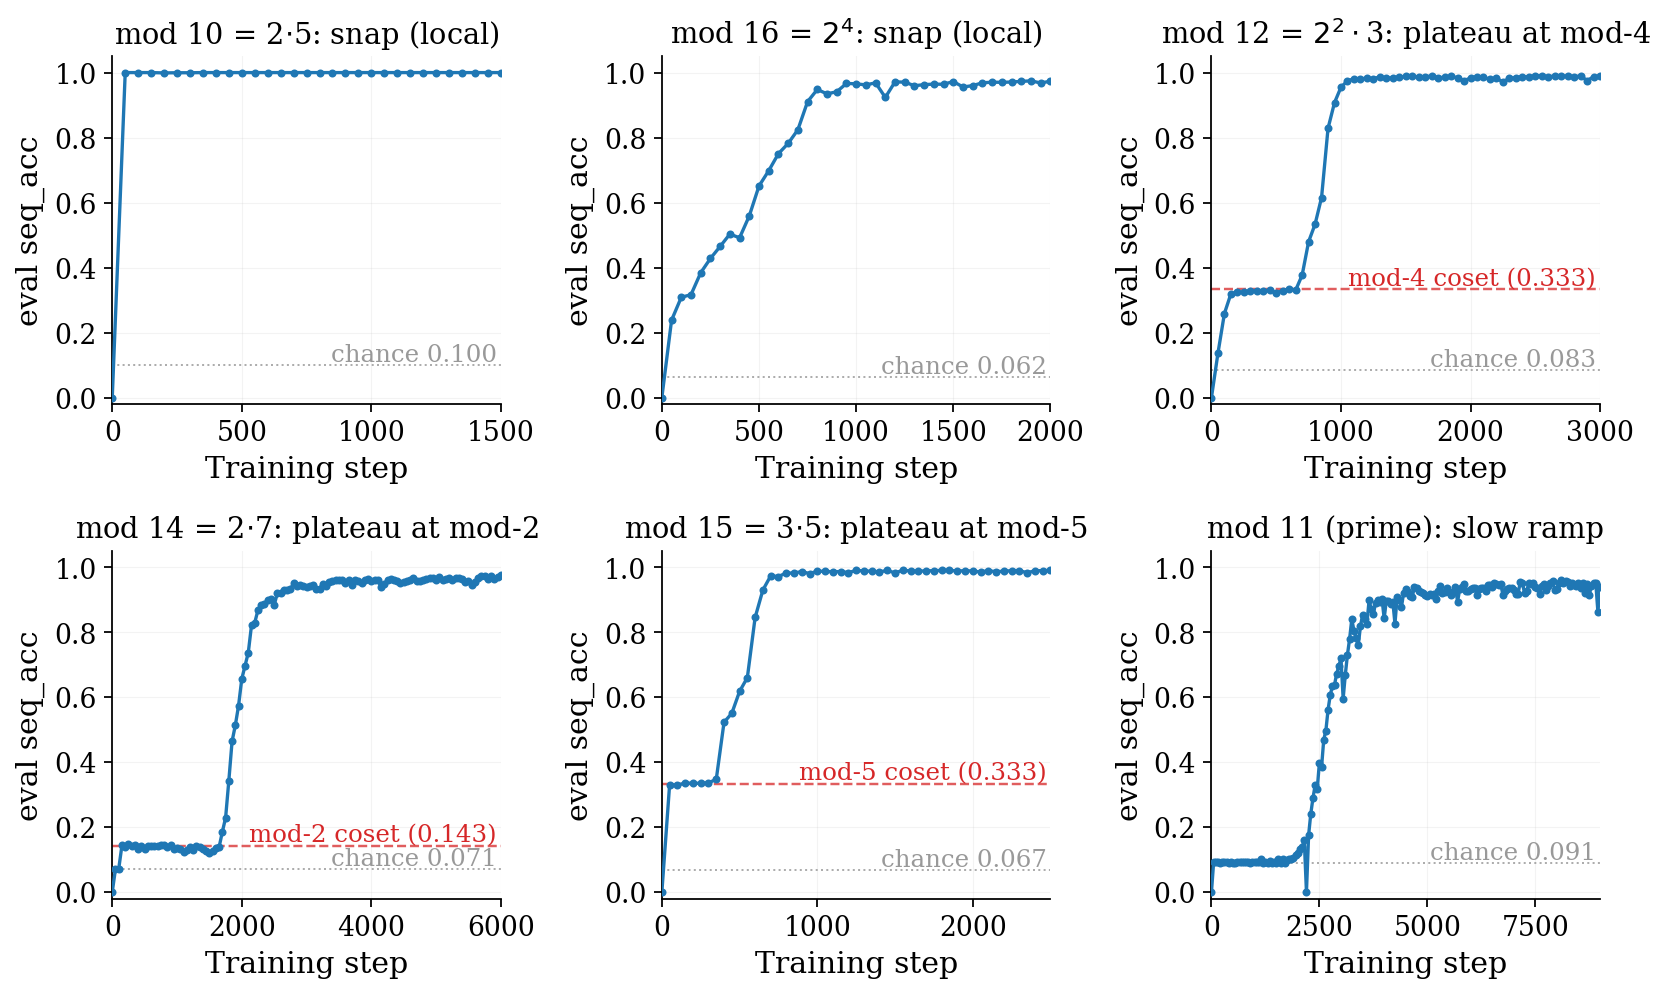
\includegraphics[width=\linewidth]{figs/moremods_test.png}
\caption{The moduli 10--16 sweep behind the law's confirmations, including the discriminating mod-10 snap and the mod-14 plateau at $1/7$.}
\label{fig:moremods}
\end{figure}

\begin{figure}[h]
\centering
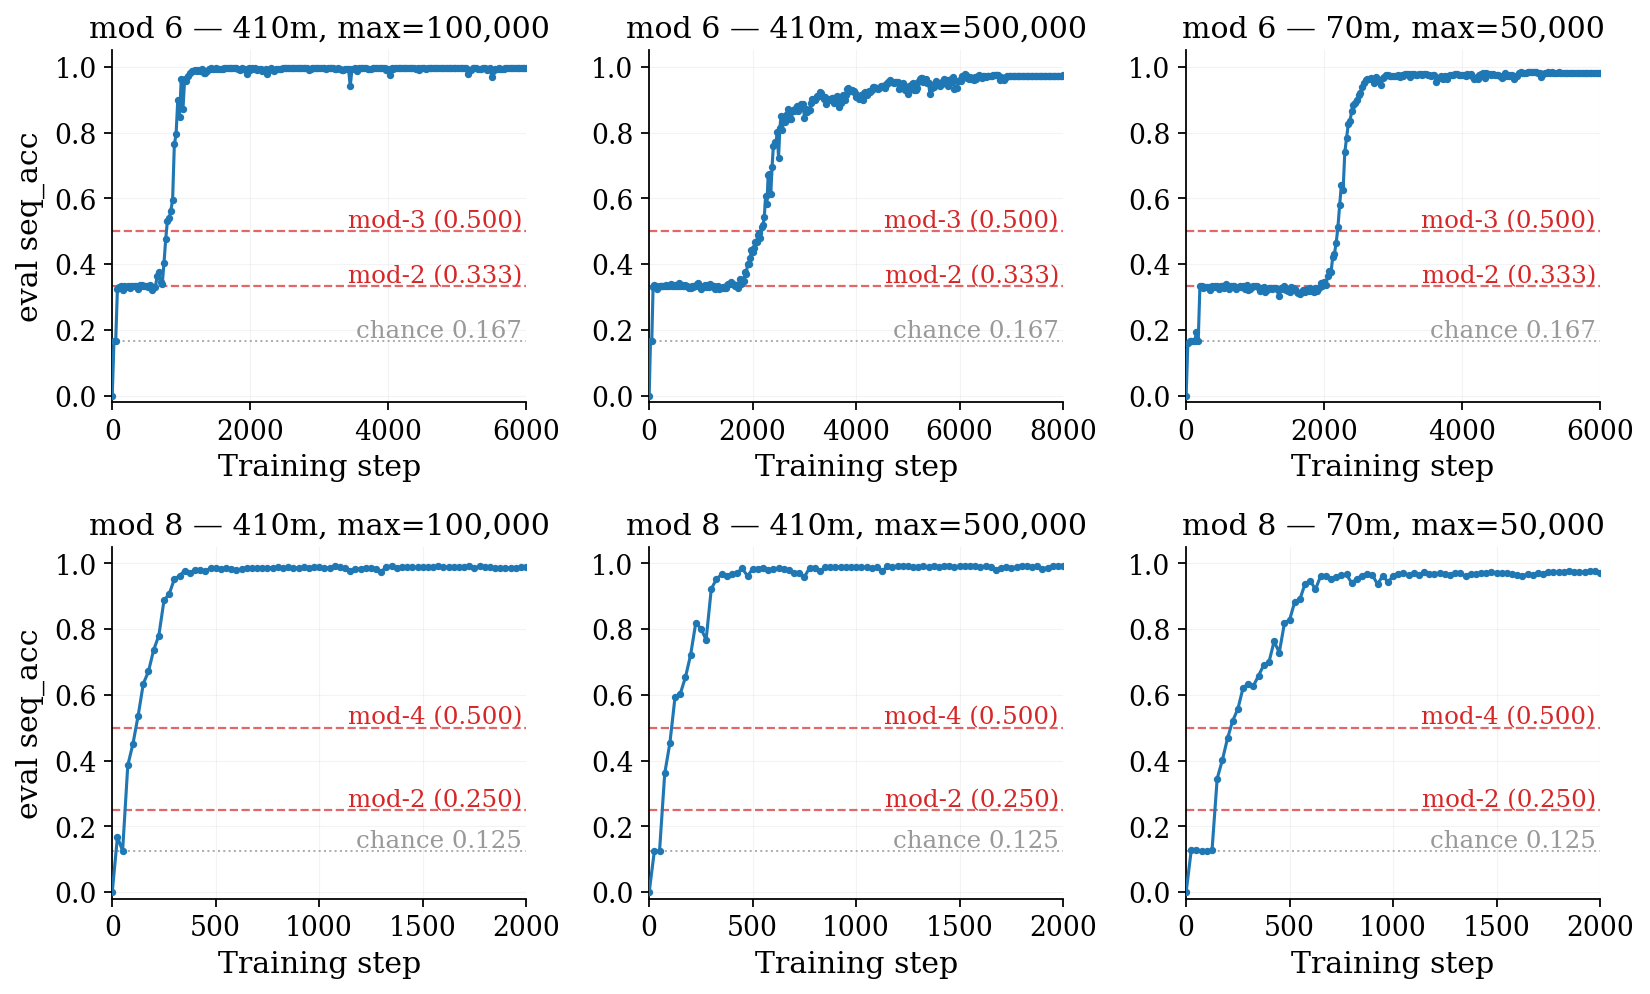
\includegraphics[width=0.9\linewidth]{figs/nimsimple_mag_size.png}
\caption{Plateau dwell scaling with operand magnitude and model size (mod 6).}
\label{fig:magsize}
\end{figure}

\section{Entrenchment detail: the donor-checkpoint sweep, the dwell-state probe, and the oracle-injection control}
\label{app:dwell}

\paragraph{The oracle-injection control in full.} During training we add $\alpha \|h\| (\cos(2\pi\,\mathrm{ds}/9)\, u_1 + \sin(2\pi\,\mathrm{ds}/9)\, u_2)$---$u_1, u_2$ a fixed random orthonormal pair---to the residual stream at layer 13, at the answer-predicting position ($\alpha \in \{0.1, 0.3\}$). Training-time results: f95 $= 125$ and $25$ respectively, no plateau, ceiling accuracy---expected, since the injected pair determines the answer. The installation-cost ladder this completes: oracle plane (25) $<$ digit-sum donor (200) $<$ scratch (3725), separating the cost of reading a handed feature, hooking a readout to one's own inherited manifold, and building everything. Saved checkpoints contain no hook, so plain evaluation measures the weights alone: \emph{chance at every checkpoint} (0.110--0.113, both amplitudes, all depths; not even the coset formed). With loss already near zero via the injected feature, no gradient pressure remains to build anything---the selection law's limiting case. The contrast with the donor route is the useful residue: donors yield \emph{ownership} (a transferable mechanism in the weights), oracles yield \emph{rental} (instant performance, zero acquisition)---and the two are indistinguishable during training, a caution for any regime in which an auxiliary signal is always available. Whether annealing $\alpha \to 0$ converts rental into ownership is future work.



\begin{figure}[h]
\centering
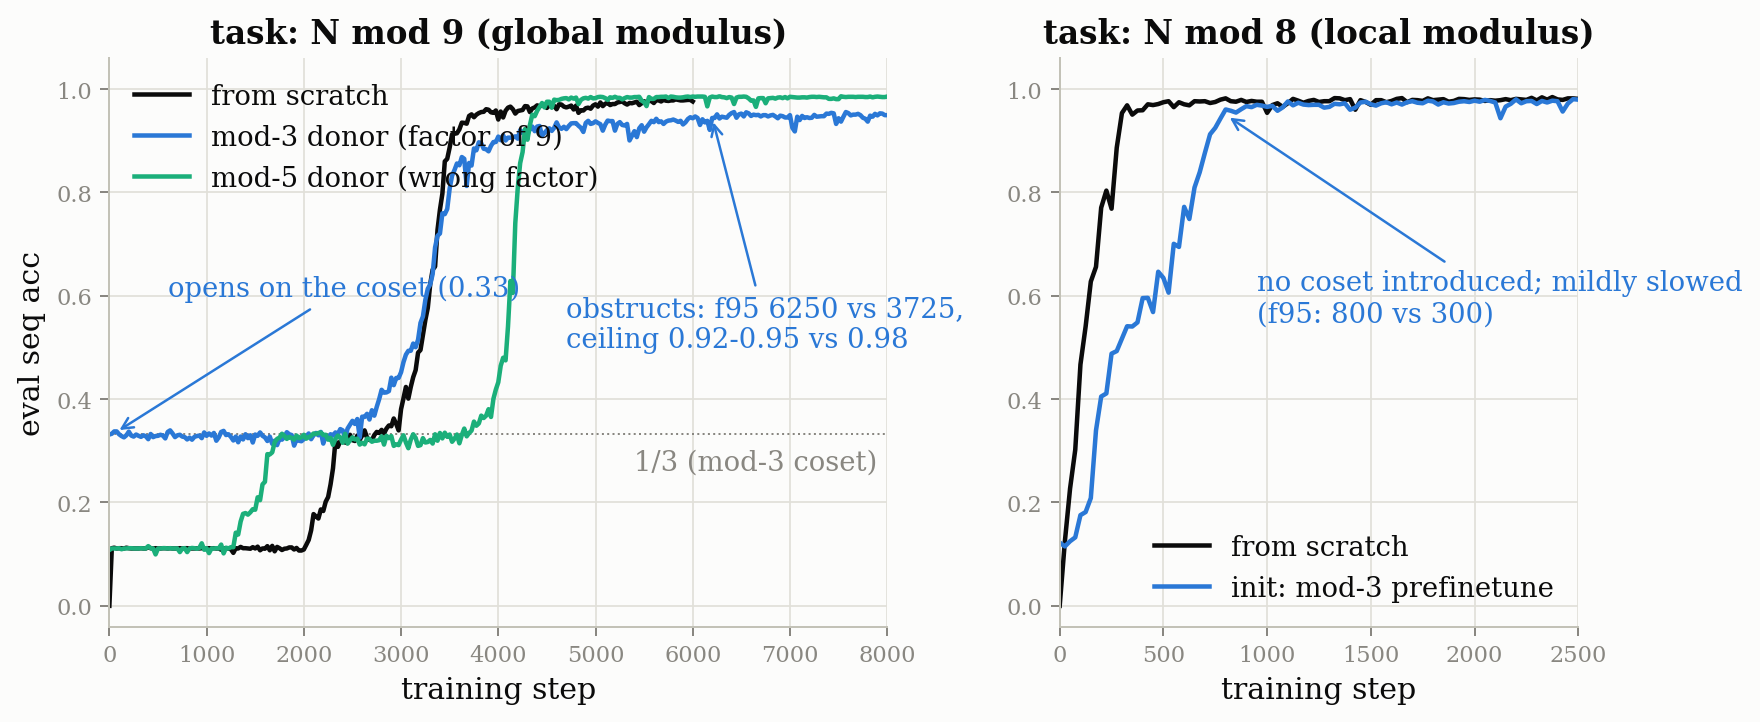
\includegraphics[width=\linewidth]{figs/install_transfer.png}
\caption{The original install experiment: mod-9 training from scratch, from the mod-3 donor (opens at $1/3$, dwells $>3\times$ the natural plateau, stalls below the ceiling), and from the mod-5 wrong-factor donor (ends best). Right: mod-8 control.}
\label{fig:install}
\end{figure}

\begin{figure}[h]
\centering
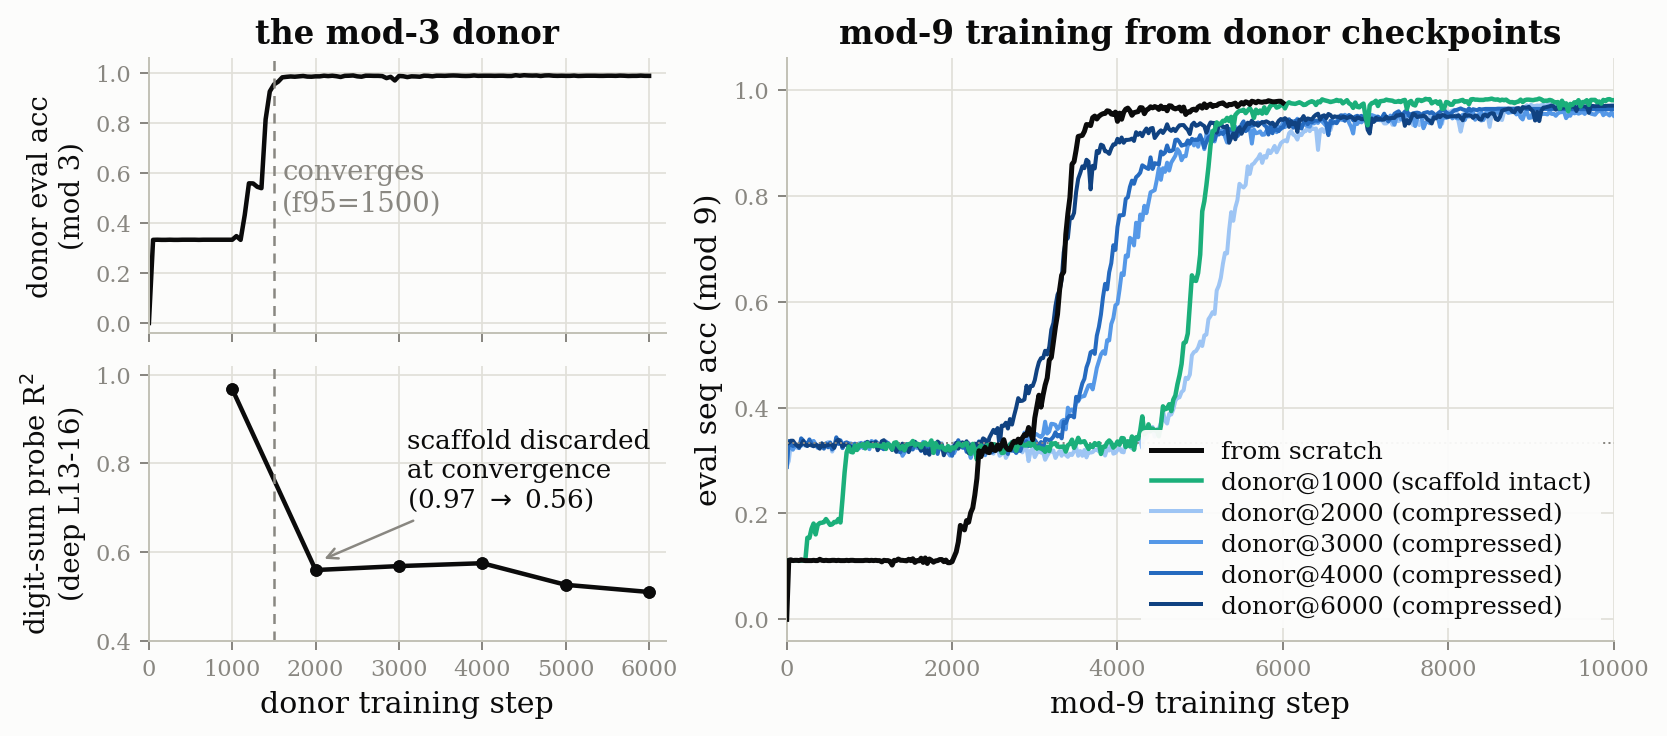
\includegraphics[width=\linewidth]{figs/install_dose.png}
\caption{\textbf{Dose-response}. Left: the donor's convergence (top) and its deep-layer digit-sum $R^2$ (bottom)---the scaffold is discarded in a step at convergence. Right: mod-9 training from donor checkpoints. No run beats scratch; at the coset all models are behaviorally identical yet differ $4$--$7\times$ in escape time. The ceiling deficit appears only in compressed-donor runs (blues); the uncompressed-donor run (green) recovers the scratch ceiling fully; the timing cost is worst for the freshly converged donor and shrinks with donor overtraining.}
\label{fig:dose}
\end{figure}

\begin{figure}[h]
\centering
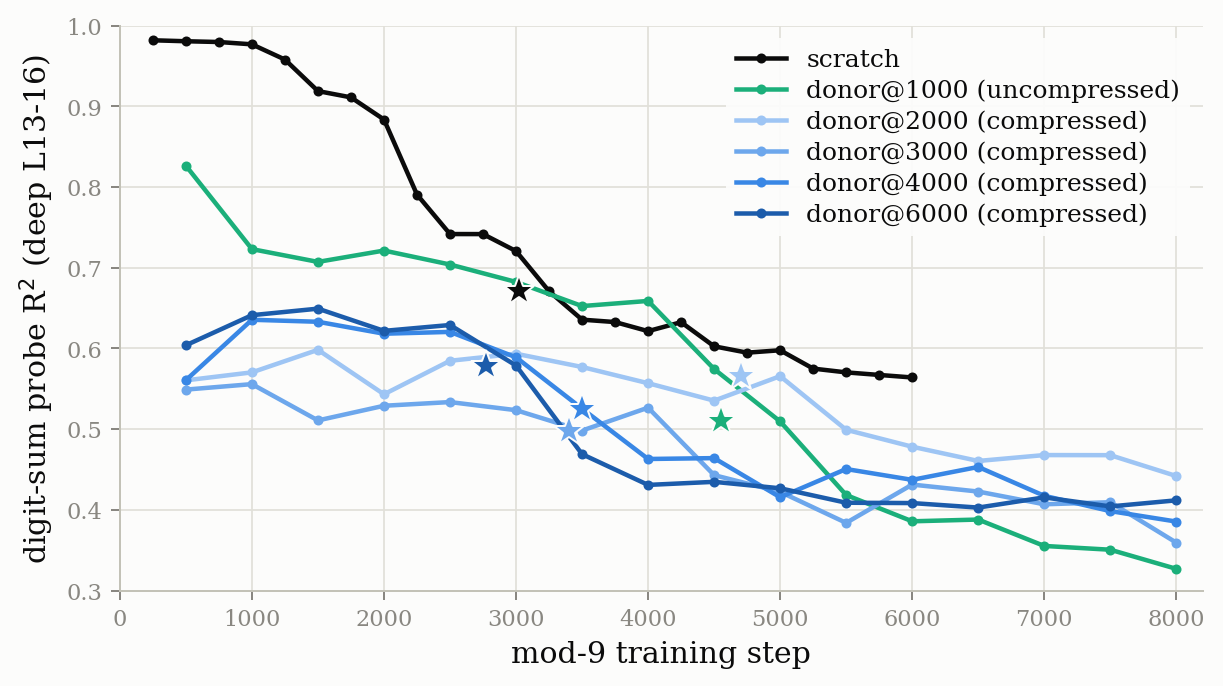
\includegraphics[width=0.85\linewidth]{figs/dwell_probe.png}
\caption{Deep-layer digit-sum $R^2$ across mod-9 training for scratch and all five donor runs; stars mark each run's escape step. No run recovers the scaffold before escaping; compression deepens through and past the climb. Cross-run rank correlation between dwell-period $R^2$ and escape time: $\rho \approx 0.31$ (pre-specified threshold 0.8).}
\label{fig:dwell}
\end{figure}

\section{Format disentanglement figure}
\label{app:disentangle}

\begin{figure}[h]
\centering
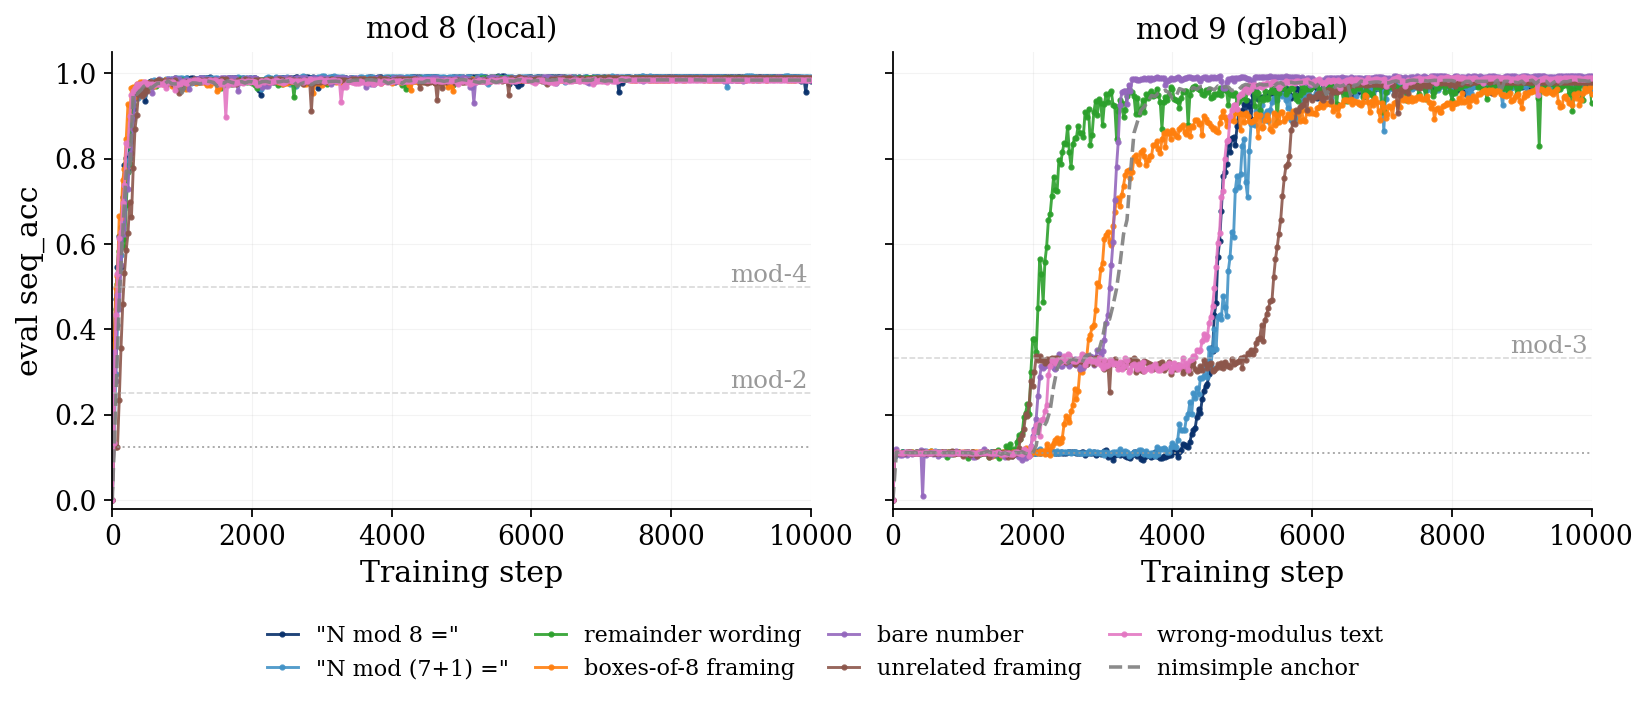
\includegraphics[width=\linewidth]{figs/disentangle.png}
\caption{All eight single-operand formats, mod 8 and mod 9, identical held-out operand pools.}
\label{fig:disentangle}
\end{figure}

\end{document}
